\part{Gestión de la tesis}
\label{part:gestion-tesis}
%%%%%%%%%%%%%%%%%%%%%%%%%%%%%%%%%%%%%%%%%%%%%%%%%%%%%%%%%%%%%%%%%

\section{Introducción y contextualización}

Los modelos de lenguaje de gran tamaño (Large Language Models, LLMs) han transformado el procesamiento del lenguaje natural en los últimos años. Modelos como LLaMA o Mistral muestran capacidades notables en generación de texto, comprensión lectora, traducción y razonamiento. Sin embargo, su entrenamiento y despliegue requieren recursos computacionales y costes de operación que dificultan su adopción fuera de organizaciones con infraestructuras significativas. Esta barrera de coste es uno de los principales obstáculos para la democratización de estas tecnologías.

El problema central que aborda este TFG puede formularse así. \textbf{¿Cómo reducir el coste computacional de inferencia de los modelos de lenguaje de gran tamaño (LLMs) sin degradar significativamente la calidad de sus respuestas?}

Este problema es relevante por varias razones. El coste elevado de inferir con LLMs grandes limita su accesibilidad a organizaciones con recursos considerables. Además, no todas las peticiones requieren la capacidad completa del modelo más potente. Muchas pueden resolverse satisfactoriamente con modelos más pequeños y eficientes. Esta observación sugiere que pueden diseñarse estrategias de asignación dinámica que seleccionen el modelo más adecuado en función de la dificultad estimada de cada petición.

Una de las aproximaciones posibles consiste en utilizar un sistema de cascada de modelos, respondiendo con el modelo pequeño cuando basta y escalando al grande solo cuando es necesario. En aplicaciones interactivas, donde el tiempo de respuesta importa, este tipo de enfoque puede mejorar la latencia media al evitar el uso del modelo grande en peticiones sencillas.

Para validar experimentalmente el equilibrio entre calidad y coste, se desplegará la propuesta en el Barcelona Supercomputing Center (BSC), concretamente en MareNostrum~5, utilizando vLLM como motor de serving. Es importante destacar que BSC y vLLM constituyen la infraestructura de experimentación y medición, no el objetivo principal del TFG. Proporcionan la plataforma para desplegar las distintas políticas de serving y registrar métricas de servicio (TTFT, latencia, throughput, memoria GPU), que se compararán con métricas de calidad en tareas NLP estándar.

\subsection{Marco institucional y encaje académico}

Este proyecto se enmarca en el Trabajo de Fin de Grado del Grado en Ingeniería Informática de la Facultat d'Informàtica de Barcelona (FIB), dentro de la especialidad de Computación. La modalidad del TFG es A. El tema aborda un problema central de la ingeniería de sistemas inteligentes, combinando arquitectura de sistemas, optimización de recursos y aprendizaje automático. El entorno de ejecución en MareNostrum~5 permite trabajar con infraestructura de supercomputación real, lo que aporta una dimensión práctica y profesionalizadora que complementa la formación teórica recibida en asignaturas como Arquitectura de Computadores, Aprendizaje Automático y Computación de Altas Prestaciones.

La colaboración con el BSC facilita el acceso a recursos de cómputo que no estarían disponibles en un entorno académico convencional. Esta colaboración permite validar las estrategias propuestas en condiciones realistas y genera resultados transferibles a otros entornos HPC o de producción con infraestructura similar.

\subsection{Actores implicados y beneficiarios}

Los usuarios del resultado serán investigadores y equipos técnicos que despliegan LLMs con restricciones de coste en entornos HPC. Los scripts y documentación podrán reutilizarse por estudiantes o investigadores del BSC en líneas similares. La operación recae sobre el autor con supervisión de los codirectores.

El coste computacional es asumido por el BSC mediante la cuota del grupo de investigación \textbf{Data Centric Computing} (con identificador bsc98 en el ms5). Los beneficiarios directos son las organizaciones que implementen cascadas similares, reduciendo uso de GPUs y consumo energético. La comunidad académica se beneficia de un pipeline documentado y reproducible.

%%%%%%%%%%%%%%%%%%%%%%%%%%%%%%%%%%%%%%%%%%%%%%%%%%%%%%%%%%%%%%%%%
% 2. JUSTIFICACIÓN, OBJETIVOS Y VISIÓN (agrupado para índice compacto)
%%%%%%%%%%%%%%%%%%%%%%%%%%%%%%%%%%%%%%%%%%%%%%%%%%%%%%%%%%%%%%%%%
\section{Justificación, objetivos y visión de la solución}

\subsection{Estado del arte y líneas de trabajo actuales}

El problema del coste de inferencia de los LLMs es hoy una línea de investigación muy activa, y la comunidad ha ido consolidando varias familias de respuestas que conviene conocer antes de presentar la propuesta de este TFG. Tres grandes bloques resumen razonablemente bien el panorama.

El primero agrupa las \textbf{técnicas de compresión de modelos}. La \textbf{cuantización} reduce la precisión numérica de los pesos (INT8, INT4) para acelerar cálculos y reducir memoria, aunque puede degradar la calidad de forma difícil de predecir. El \textbf{pruning} elimina conexiones redundantes para obtener modelos sparse más eficientes, pero requiere reentrenamiento y no siempre es compatible con hardware estándar. Técnicas de \textbf{PEFT} (\textit{parameter-efficient fine-tuning}), como LoRA, permiten adaptar modelos grandes con pocos parámetros entrenables, pero no reducen el coste de inferencia del modelo base. Una línea distinta, y la que se adopta en este TFG, es la de \textbf{Knowledge Distillation}~\cite{hinton2015distilling}, donde un modelo grande (teacher) transfiere conocimiento a uno más pequeño (student), que después se sirve a un coste muy inferior.

El segundo bloque es el de los \textbf{sistemas de serving eficiente}. Aquí el exponente más relevante es vLLM~\cite{vllm-docs}, un motor de inferencia con \emph{continuous batching} y \emph{PagedAttention}~\cite{vllm2023} que ha mejorado drásticamente el \textit{throughput} alcanzable con modelos medianos y grandes. Otras piezas del mismo bloque son FlashAttention~\cite{dao2022flashattention}, el \textit{speculative decoding}~\cite{leviathan2023speculative} y optimizaciones de bajo nivel sobre la atención. En este TFG, vLLM se usa como plataforma común de despliegue y medición, para que las comparaciones entre políticas se hagan en igualdad de condiciones.

El tercer bloque, más reciente y el que conecta directamente con la propuesta, es el de los \textbf{sistemas de decisión o routing entre modelos}, es decir, trabajar no con un único modelo sino con un conjunto de modelos de distinto tamaño y decidir, para cada petición, cuál es el más adecuado. FrugalGPT~\cite{chen2023frugalgpt} populariza la idea de cascada con verificación, y RouteLLM~\cite{dekoninck2024routing} explora el entrenamiento de un router que estima a priori qué modelo debería responder. El TFG se sitúa en este tercer bloque y, concretamente, propone usar KD para \emph{generar} el student que alimenta el sistema y después comparar, sobre la misma infraestructura de serving, tres políticas (\textbf{Política~A} en modo baseline, que sirve siempre con el teacher; \textbf{Política~B} en cascada forzada, que intenta primero con el modelo más pequeño y escala al grande si el resultado no pasa un filtro de calidad; y \textbf{Política~C} en cascada por confianza, que con un predictor externo decide \textit{a priori} qué modelo responde). La contribución del TFG es, por tanto, no tanto inventar una técnica nueva como \textbf{medir rigurosamente el trade-off entre calidad y coste} que esta combinación permite, en un entorno HPC real (MareNostrum~5) y con un protocolo de evaluación unificado.

\subsection{Relevancia práctica}

Reducir el coste de inferencia de LLMs es una prioridad en centros de investigación con recursos HPC compartidos y en organizaciones que despliegan asistentes conversacionales o sistemas de análisis de texto. Estas organizaciones buscan optimizar el uso de GPUs sin degradar la experiencia de usuario. Las cascadas de modelos responden a esta necesidad, usando el modelo pequeño cuando basta y escalando al grande solo cuando es necesario. Aunque el proyecto se ejecuta en MareNostrum~5 del BSC, los resultados son transferibles a otros entornos HPC o de producción con infraestructura similar.

\subsection{Relevancia académica}

El proyecto contribuye al ámbito académico mediante la documentación de un pipeline reproducible de evaluación, el análisis comparativo del balance entre calidad y eficiencia para las políticas mínimas A y B (y C si es viable), y la exploración de mecanismos de routing basados en confianza, un área con literatura emergente~\cite{chen2023frugalgpt, dekoninck2024routing}.

\subsection{Análisis de alternativas y decisión de diseño}

Se consideraron tres alternativas para reducir el coste de inferencia.

\textbf{Alternativa~1 (cuantización del teacher, INT8/INT4).} Reduce memoria y acelera inferencia sin modelos adicionales. Riesgo técnico bajo, pero ganancia limitada al factor de compresión y degradación difícil de controlar.

\textbf{Alternativa~2 (solo modelos pequeños preentrenados, contingencia).} Implementación sencilla, sin lógica de decisión. Riesgo muy bajo, pero calidad fija y sin flexibilidad para escalar en peticiones complejas.

\textbf{Alternativa~3 (elegida, sistema de cascada con múltiples políticas).} Combina modelos de distintos tamaños y compara políticas de serving (baseline, cascada forzada, cascada por confianza). Mayor complejidad, pero es la única que permite estudiar experimentalmente el equilibrio entre calidad y coste, objetivo central del TFG.

La Tabla~\ref{tab:alternativas} resume los puntos fuertes y débiles de cada alternativa.

\begin{table}[H]
\centering
\caption{Comparación de alternativas de diseño. Fuente: elaboración propia.}
\label{tab:alternativas}
\footnotesize
\begin{tabularx}{\textwidth}{>{\raggedright\arraybackslash}p{2.8cm} >{\raggedright\arraybackslash}X >{\raggedright\arraybackslash}X >{\raggedright\arraybackslash}p{3cm}}
\toprule
\textbf{Alternativa} & \textbf{Puntos fuertes} & \textbf{Puntos débiles} & \textbf{Encaje con el TFG} \\
\midrule
1. Cuantización del teacher & Bajo riesgo técnico; sin modelos adicionales; ganancia directa en memoria e inferencia & Ganancia limitada al factor de compresión; degradación de calidad difícil de controlar & Parcial: mejora eficiencia pero no permite analizar routing \\
\addlinespace
2. Solo modelos pequeños & Implementación sencilla; sin lógica de decisión & Calidad fija; sin flexibilidad ante peticiones complejas & Bajo: no aborda el equilibrio dinámico calidad--coste \\
\addlinespace
3. Cascada (elegida) & Permite comparar políticas de serving; estudia experimentalmente el equilibrio calidad--coste & Mayor complejidad de implementación y evaluación & Alto: responde directamente a la pregunta de investigación \\
\bottomrule
\end{tabularx}
\end{table}

Se adopta la tercera alternativa porque responde a la pregunta de investigación y mantiene como eje el marco entre \textit{teacher} y \textit{student} mediante knowledge distillation. Las otras resuelven parcialmente la eficiencia pero no permiten analizar el comportamiento dinámico de la cascada ni la comparación de políticas. Con acceso a MareNostrum~5, la complejidad adicional es asumible.

\subsection{Objetivo general}

El proyecto se estructura en torno a un objetivo principal y seis objetivos específicos (OE1--OE6), cada uno con criterios de aceptación cuantitativos y auditables.

El objetivo general de este TFG es \textbf{diseñar, implementar y evaluar un sistema de inferencia de LLMs basado en cascada de modelos entre \textit{teacher} y \textit{student}}, comparando experimentalmente las políticas mínimas de serving (baseline y cascada forzada) e incorporando la cascada por confianza si resulta viable, para analizar el equilibrio entre calidad y coste mediante despliegue en MareNostrum~5.

\subsection{Objetivos específicos y criterios de aceptación}
\label{subsec:oe-especificos}

A continuación, se detallan los objetivos específicos (OE1--OE6) con sus criterios de aceptación auditables.

\textbf{OE1. Desplegar infraestructura de serving con vLLM.}\\
Configurar y ejecutar modelos como servidores de inferencia en MareNostrum~5 usando vLLM.\\
\textit{Indicador:} servidor operativo sin errores críticos (caída, HTTP~5xx sostenidos, OOM).\\
\textit{Método:} revisión de logs del servidor (\texttt{vllm.log}).\\
\textit{Condición mínima:} 1~hora de ejecución continua tras warmup de 5~minutos.\\
\textit{Umbral de éxito:} 0~errores críticos en la ventana de medida.

\textbf{OE2. Diseñar generador de peticiones y recolección de datos.}\\
Implementar scripts Python que envíen peticiones, recojan respuestas con metadatos (tiempos, tokens, log~probs) y almacenen resultados.\\
\textit{Indicador:} fichero de resultados completo.\\
\textit{Método:} script \texttt{benchmark\_client.py} exportando a JSON/CSV.\\
\textit{Condición mínima:} 100~peticiones consecutivas sin pérdida de datos.\\
\textit{Umbral de éxito:} 100\% de respuestas registradas con metadatos (timestamp, TTFT, latencia, tokens).

\textbf{OE3. Medir métricas de servicio.}\\
Registrar Time To First Token (TTFT), latencia total, throughput (tokens/s) y memoria GPU para al menos dos configuraciones de modelo.\\
\textit{Indicador:} ficheros de métricas con p50 y p95.\\
\textit{Método:} script de análisis sobre logs; memoria vía \texttt{nvidia-smi}.\\
\textit{Condición mínima:} 3~repeticiones por configuración, warmup de 10~peticiones, misma config de decoding.\\
\textit{Umbral de éxito:} disponer de p50, p95 y throughput medio para $\geq2$ configuraciones.

\textbf{OE4. Evaluar calidad en tareas de razonamiento matemático.}\\
Medir calidad en GSM8K y MATH usando exact match sobre la respuesta final.\\
\textit{Indicador:} métricas de calidad (accuracy/EM) documentadas para ambos benchmarks.\\
\textit{Método:} \texttt{lm-evaluation-harness} o scripts propios comparando con ground truth.\\
\textit{Condición mínima:} evaluación en GSM8K y MATH, misma plantilla de prompt, temperatura y top\_p fijos.\\
\textit{Umbral de éxito:} informe con accuracy/EM para GSM8K y MATH.

\textbf{OE5. Obtener modelos student para la cascada.}\\
La vía principal es obtener un student mediante knowledge distillation del teacher; solo si la ejecución no es viable con la cuota disponible, seleccionar un modelo preentrenado equivalente como contingencia y documentar la decisión.\\
\textit{Indicador:} modelo student desplegado y operativo.\\
\textit{Método:} despliegue con vLLM y prueba de inferencia.\\
\textit{Condición mínima:} al menos 1~student funcional.\\
\textit{Umbral de éxito:} student responde correctamente a 100~peticiones de prueba.

\textbf{OE6. Implementar y evaluar políticas de cascada.}\\
Implementar la Política~B (cascada forzada) como mínimo exigible y la Política~C (cascada por confianza) si los recursos lo permiten. Comparar ambas contra la Política~A (baseline).\\
\textit{Indicador:} reducción de uso del teacher manteniendo calidad.\\
\textit{Método:} comparar políticas en el mismo conjunto de prueba.\\
\textit{Condición mínima:} Política~A y Política~B evaluadas con 3~repeticiones.\\
\textit{Umbral de éxito:} Política~B reduce $\geq$20\% las peticiones al teacher sin degradar calidad más de 5~puntos porcentuales respecto a Política~A.

\subsection{Descripción general de la solución}

La solución se estructura en siete fases técnicas. En la \textbf{Fase~1} se selecciona y despliega el modelo teacher con vLLM, que proporciona un servidor HTTP con PagedAttention~\cite{vllm2023}. En la \textbf{Fase~2} se implementa la generación de peticiones y recolección de datos (tiempos, tokens, log~probs) mediante scripts Python. En la \textbf{Fase~3} se miden métricas de servicio (TTFT, latencia, throughput, memoria GPU). En la \textbf{Fase~4} se evalúa el teacher en los benchmarks seleccionados para establecer la referencia de calidad (Política~A).

\begin{figure}[H]
\centering
\resizebox{\textwidth}{!}{%
\begin{tikzpicture}[
>=Latex,
node distance=8mm and 14mm,
sys/.style={draw, rounded corners=2.2pt, align=center, minimum width=3.1cm, minimum height=9mm, font=\small, thick},
flow/.style={->, thick}
]
\node[sys, fill=yellow!18] (req) {Petición de usuario};
\node[sys, right=of req, fill=orange!20] (router) {Módulo de routing};

\node[sys, above right=10mm and 14mm of router, fill=blue!16] (student) {Student};
\node[sys, below right=10mm and 14mm of router, fill=red!14] (teacher) {Teacher};

\node[sys, right=45mm of router, fill=gray!14, minimum width=3cm] (merge) {Output};
\node[sys, right=of merge, fill=teal!16, minimum width=4.0cm] (metrics) {Registro de métricas\\TTFT, latencia, throughput, EM};

\draw[flow] (req) -- (router);
\draw[flow] (router) -- node[above, sloped, font=\tiny, align=center] {petición\\simple} (student);
\draw[flow] (router) -- node[below, sloped, font=\tiny, align=center] {petición\\compleja} (teacher);
\draw[flow] (student) -- node[right, font=\tiny, align=center] {cascada} (teacher);
\draw[flow] (student.east) -- ++(7mm,0) |- (merge.north west);
\draw[flow] (teacher.east) -- ++(7mm,0) |- (merge.south west);
\draw[flow] (merge) -- (metrics);

\begin{scope}[on background layer]
\node[draw=orange!45, rounded corners=4pt, fill=orange!5, fit=(router)(student)(teacher), inner sep=6pt] {};
\end{scope}
\end{tikzpicture}%
}%resizebox
\caption{Arquitectura operativa del sistema de cascada: enrutado por dificultad, fallback al teacher y trazabilidad de métricas. Fuente: elaboración propia.}
\label{fig:arquitectura-sistema}
\end{figure}

\textbf{Benchmarks seleccionados (GSM8K y MATH).} Se han elegido dos benchmarks de razonamiento matemático~\cite{cobbe2021gsm8k, hendrycks2021math}. GSM8K contiene problemas de aritmética escolar con razonamiento en varios pasos; MATH incluye problemas de competición de mayor dificultad. Ambos permiten medir si el modelo pequeño resuelve problemas sencillos y si el routing detecta cuándo escalar al grande. La métrica es \textit{exact match} (EM) sobre la respuesta final.

En la \textbf{Fase~5} se selecciona al menos un student y se obtiene su línea base aplicando el mismo protocolo de evaluación que al teacher. La planificación prioriza la destilación entre \textit{teacher} y \textit{student} como núcleo metodológico; si esta no resulta viable por restricciones de cuota, se activa la contingencia con un modelo preentrenado equivalente y se documenta explícitamente. En la \textbf{Fase~6} se implementan y evalúan las políticas de cascada. La Política~B (cascada forzada) es el mínimo exigible y consiste en intentar primero con el modelo más pequeño y escalar si no cumple el criterio. La Política~C (cascada por confianza) utiliza un componente predictivo basado en señales como log~probs o entropía para decidir a priori qué modelo servir, evitando escalados innecesarios. La Política~C es la versión avanzada, viable si los recursos lo permiten, pero no es requisito indispensable del éxito del proyecto.

En la \textbf{Fase~7} se consolidan los resultados y se cierra la documentación del proyecto. Esto comprende la preparación de los scripts y configuraciones reproducibles (README, entornos y ejemplos de ejecución), la redacción final de la memoria del TFG y la preparación del material de defensa.

%%%%%%%%%%%%%%%%%%%%%%%%%%%%%%%%%%%%%%%%%%%%%%%%%%%%%%%%%%%%%%%%%
% 5. ALCANCE
%%%%%%%%%%%%%%%%%%%%%%%%%%%%%%%%%%%%%%%%%%%%%%%%%%%%%%%%%%%%%%%%%
\section{Alcance}

\subsection{Elementos incluidos y excluidos}

La Tabla~\ref{tab:scope} detalla qué elementos están dentro y fuera del alcance del proyecto.

\begin{table}[H]
\centering
\caption{Alcance del proyecto: elementos incluidos y excluidos. Fuente: elaboración propia.}
\label{tab:scope}
\small
\begin{tabular}{>{\raggedright\arraybackslash}p{6.5cm} >{\raggedright\arraybackslash}p{6.5cm}}
\toprule
\textbf{Incluido (IN scope)} & \textbf{Excluido (OUT of scope)} \\
\midrule
Despliegue de 1 o 2 modelos teacher con vLLM & Entrenamiento de LLMs desde cero \\
\addlinespace
Obtención de student por destilación entre \textit{teacher} y \textit{student} (con alternativa preentrenada solo como contingencia) & Optimización a nivel de kernel CUDA \\
\addlinespace
Implementación de Política~A (baseline) y Política~B (cascada forzada) & Desarrollo de nuevas arquitecturas de modelos \\
\addlinespace
Exploración de Política~C (cascada por confianza) si recursos lo permiten & Sistema de routing en producción con alta disponibilidad \\
\addlinespace
Medición de métricas de serving (TTFT, latencia, throughput, memoria GPU) & Cobertura exhaustiva de todos los benchmarks existentes \\
\addlinespace
Evaluación de calidad en GSM8K y MATH & Fine-tuning extensivo con múltiples técnicas \\
\addlinespace
Documentación y scripts reproducibles & Interfaz de usuario gráfica \\
\addlinespace
Análisis en entorno BSC con recursos asignados & Despliegue en cloud comercial (AWS, GCP, Azure) \\
\bottomrule
\end{tabular}
\end{table}

\subsection{Entregables}

Los entregables constituyen los resultados verificables del proyecto. Permiten cerrar el alcance de forma auditable y dan soporte a la trazabilidad entre objetivos, tareas y validación. Incluyen documentación técnica y artefactos de código.

\textbf{D1. Informe de configuración.} Documentación del despliegue de vLLM en BSC (entorno, dependencias, scripts).

\textbf{D2. Scripts de generación de peticiones.} Código Python para enviar peticiones y registrar metadatos.

\textbf{D3. Scripts de evaluación de métricas.} Herramientas para calcular métricas de servicio y calidad.

\textbf{D4. Informe comparativo de políticas.} Análisis cuantitativo del equilibrio calidad--eficiencia para A y B, incorporando C si su implementación es viable, y contraste entre \textit{teacher} y \textit{student}.

\textbf{D5. Prototipo de cascada.} Implementación y evaluación de la cascada entre \textit{teacher} y \textit{student} (con contingencia preentrenada, si aplica).

\textbf{D6. Memoria final del TFG.} Documento completo con metodología, experimentos, resultados y conclusiones.

\textbf{D7. Repositorio de código.} Código fuente organizado y documentado en Git.

\subsection{Matriz de trazabilidad}

La Tabla~\ref{tab:trace} relaciona objetivos, entregables, criterios y evidencias verificables.

\begin{table}[H]
\centering
\caption{Trazabilidad OE $\leftrightarrow$ entregables $\leftrightarrow$ evidencia. Fuente: elaboración propia.}
\label{tab:trace}
\footnotesize
\setlength{\tabcolsep}{3pt}
\begin{tabularx}{\textwidth}{>{\raggedright\arraybackslash}p{0.8cm} >{\raggedright\arraybackslash}p{1.8cm} X >{\raggedright\arraybackslash}p{3.8cm}}
\toprule
\textbf{OE} & \textbf{Entregables} & \textbf{Criterio resumido} & \textbf{Evidencia verificable} \\
\midrule
OE1 & D1, D7 & Servidor 1h sin errores críticos & \texttt{vllm.log} sin OOM/5xx \\
OE2 & D2, D7 & 100 peticiones registradas & \texttt{results.json} con 100 filas completas \\
OE3 & D3, D4 & Métricas p50/p95 para $\geq$2 configs & Ficheros CSV con TTFT, latencia, throughput \\
OE4 & D3, D4, D6 & Calidad en GSM8K y MATH & Tabla con accuracy/EM por benchmark \\
OE5 & D1, D4, D7 & Student obtenido por distilación (o contingencia justificada), desplegado y operativo & Log de 100 respuestas del student y registro de decisión técnica \\
OE6 & D5, D6 & Política~B reduce $\geq$20\% uso teacher, $\leq$5pp pérdida & Tabla comparativa políticas A, B (y C si viable) \\
\bottomrule
\end{tabularx}
\end{table}

\subsection{Requisitos operativos y criterios de aceptación}

Dado que este TFG no desarrolla un producto software convencional, sino un pipeline experimental de evaluación, los requisitos funcionales y no funcionales tradicionales no aplican de forma directa. En su lugar, los criterios de aceptación definidos para cada objetivo específico (Sección~\ref{subsec:oe-especificos}) actúan como requisitos operativos del pipeline, estableciendo condiciones cuantitativas que la infraestructura, los scripts y el protocolo experimental deben satisfacer para considerar válido cada entregable. Esta formulación es coherente con la naturaleza experimental del proyecto, donde la calidad se mide por la reproducibilidad y la trazabilidad de los resultados, no por funcionalidades de usuario final.

Los criterios detallados se encuentran en la Sección~\ref{subsec:oe-especificos} junto a cada objetivo específico. La Tabla~\ref{tab:acceptance} ofrece una vista resumida.

\begin{table}[H]
\centering
\caption{Resumen de requisitos operativos y criterios de aceptación. Fuente: elaboración propia.}
\label{tab:acceptance}
\footnotesize
\setlength{\tabcolsep}{4pt}
\begin{tabularx}{\textwidth}{>{\raggedright\arraybackslash}p{1cm} X >{\raggedright\arraybackslash}p{4.5cm}}
\toprule
\textbf{OE} & \textbf{Criterio} & \textbf{Evidencia} \\
\midrule
OE1 & Servidor 1h sin errores críticos (OOM, 5xx) & Log \texttt{vllm.log} \\
OE2 & 100 peticiones registradas con metadatos & \texttt{results.json} \\
OE3 & p50/p95 TTFT, latencia, throughput para $\geq$2 configs & Ficheros CSV \\
OE4 & Accuracy/EM en GSM8K y MATH & Tabla comparativa por benchmark \\
OE5 & Student por distilación (o contingencia justificada) desplegado y operativo (100 respuestas) & Log de respuestas y decisión documentada \\
OE6 & Política~B reduce $\geq$20\% uso teacher, $\leq$5pp pérdida & Tabla comparativa políticas \\
\bottomrule
\end{tabularx}
\end{table}

\subsection{Restricciones y supuestos}

\textbf{Restricciones.} Ejecución en BSC sujeta a políticas SLURM y cuota GPU asignada. Posibles restricciones de red para servicios HTTP. Dependencia de versiones compatibles vLLM/PyTorch/CUDA. Duración limitada (un cuatrimestre).

\textbf{Supuestos.} Acceso a modelos públicos (LLaMA~\cite{touvron2023llama}, Mistral~\cite{jiang2023mistral}) y datasets gratuitos. Compatibilidad vLLM con modelos seleccionados. La destilación entre \textit{teacher} y \textit{student} es la vía principal; si resulta inviable, se activará la contingencia con modelos preentrenados pequeños equivalentes.

\subsection{Riesgos iniciales y mitigación}

La identificación temprana de riesgos forma parte del alcance porque condiciona directamente los objetivos y las decisiones de diseño. La Tabla~\ref{tab:risks} presenta los riesgos identificados con disparadores, responsables y planes de contingencia.

\begin{table}[H]
\centering
\caption{Riesgos, disparadores, responsables y contingencia. Fuente: elaboración propia.}
\label{tab:risks}
\scriptsize
\setlength{\tabcolsep}{2pt}
\begin{tabularx}{\textwidth}{>{\raggedright\arraybackslash}p{2cm} c c >{\raggedright\arraybackslash}p{2.2cm} c >{\raggedright\arraybackslash}X}
\toprule
\textbf{Riesgo} & \textbf{Prob.} & \textbf{Imp.} & \textbf{Disparador} & \textbf{Resp.} & \textbf{Plan B / Contingencia} \\
\midrule
Colas GPU saturadas & Media & Alto & Espera $>$48h & Est. & Ejecutar en baja demanda; priorizar experimentos críticos. \\
\addlinespace
Destilación inviable & Media & Alto & Cuota GPU insuficiente & Est. & Activar contingencia con modelo preentrenado equivalente y documentar intento de destilación. \\
\addlinespace
Señal de confianza no discrimina & Media & Medio & Router no distingue aciertos/fallos & Est. & Probar entropía u otras señales; aceptar Política~B como resultado válido. \\
\addlinespace
Predictor no generaliza & Media & Medio & Precisión $<$60\% en validación & Est. & Simplificar modelo predictivo; priorizar Política~B como resultado mínimo. \\
\addlinespace
Latencia extra del routing & Media & Medio & Overhead $>$10\% de latencia base & Est. & Optimizar predictor; documentar overhead como parte del análisis. \\
\addlinespace
Errores de calibración & Media & Medio & Confianza no correlaciona con acierto & Est. & Aplicar calibración post-hoc; aceptar resultado exploratorio. \\
\addlinespace
Complejidad multi-modelo & Media & Medio & Errores al servir varios modelos & Est. & Simplificar a 2 modelos; serializar si hay conflictos de memoria. \\
\addlinespace
Incompatibilidad software & Baja & Medio & Error vLLM/PyTorch & Est. & Usar versiones alternativas; consultar soporte BSC. \\
\bottomrule
\end{tabularx}
\end{table}

%%%%%%%%%%%%%%%%%%%%%%%%%%%%%%%%%%%%%%%%%%%%%%%%%%%%%%%%%%%%%%%%%
% 6. METODOLOGÍA, DATOS Y RECURSOS (agrupado)
%%%%%%%%%%%%%%%%%%%%%%%%%%%%%%%%%%%%%%%%%%%%%%%%%%%%%%%%%%%%%%%%%
\section{Metodología, datos y recursos del proyecto}
\label{sec:metodologia-trabajo}

\subsection{Enfoque metodológico}

Se seguirá \textbf{Scrum adaptado} con sprints de dos semanas, complementado con un \textbf{tablero Kanban} (To~do / Doing / Done) para el seguimiento diario del flujo de tareas~\cite{schwaber2020scrum}. Scrum adaptado encaja en un TFG experimental porque el ciclo de iterar, medir y decidir es inherente al trabajo, ya que los resultados de cada experimento condicionan los siguientes pasos y las iteraciones cortas permiten incorporar hallazgos antes de comprometer más recursos. El tablero Kanban proporciona visibilidad continua sobre el estado de cada tarea e identifica bloqueos (por ejemplo, esperas en colas GPU) sin necesidad de esperar a la revisión de sprint. Además, al tratarse de un proyecto unipersonal, Scrum se adapta simplificando las ceremonias al mínimo operativo que aporta valor real.

\textbf{Ceremonias.}
\begin{itemize}[nosep,leftmargin=*]
\item \textbf{Sprint Planning (inicio de sprint):} seleccionar tareas del Product Backlog derivado del WBS de este documento, definir el objetivo del sprint y establecer qué métricas o evidencias validan su cumplimiento.
\item \textbf{Seguimiento semanal:} revisar bloqueos y avance contra el Sprint Backlog. Las reuniones quincenales con la codirección actúan como punto de control externo; en las semanas intermedias, la revisión es individual sobre el tablero Kanban.
\item \textbf{Sprint Review (final de sprint):} presentar los resultados medibles del sprint (tablas, CSV, logs, scripts) y compararlos con los criterios de aceptación definidos en los objetivos específicos (Sección~\ref{subsec:oe-especificos}).
\item \textbf{Retrospectiva:} registrar qué aspectos del proceso o de los experimentos se pueden mejorar y ajustar el backlog en consecuencia.
\end{itemize}

\textbf{Artefactos.}
\begin{itemize}[nosep,leftmargin=*]
\item \textbf{Product Backlog:} lista priorizada de tareas derivada del WBS definido en este documento. Cada entrada está ligada a un objetivo específico (OE1--OE6) y a un entregable (D1--D7).
\item \textbf{Sprint Backlog:} subconjunto de tareas seleccionadas para el sprint en curso, con estado visible en el tablero Kanban.
\item \textbf{Evidencias:} resultados reproducibles generados por cada tarea: scripts, configuraciones, logs de ejecución, tablas de métricas y gráficos.
\item \textbf{CHANGELOG / registro de decisiones:} fichero \texttt{CHANGELOG.md} que documenta qué se cambió y por qué en cada iteración, asegurando la trazabilidad de las decisiones de diseño.
\end{itemize}

\textbf{Definition of Done.} Una tarea se considera terminada cuando cumple todos los criterios siguientes.
\begin{enumerate}[nosep,leftmargin=*]
\item Código, scripts o configuración commitados en el repositorio Git y ejecución reproducible desde cero.
\item Métricas o resultados guardados en formato persistente (CSV, JSON o log) y referenciados desde la tarea.
\item Breve interpretación del resultado documentada (en el issue o en \texttt{CHANGELOG.md}).
\item Checklist de la tarea marcada como completada y vinculada al milestone correspondiente.
\end{enumerate}

\textbf{Conexión con la planificación temporal.} El diagrama de Gantt y el WBS definidos en este documento constituyen el macro-plan del proyecto, organizando las fases (F1--F7) y tareas transversales (TG) con sus dependencias y fechas objetivo. Los sprints de dos semanas ejecutan ese plan: en cada Sprint Planning se seleccionan tareas del WBS según prioridad y dependencias. Si se producen desviaciones, se replanifica el backlog de los sprints siguientes manteniendo los objetivos y restricciones del proyecto.

\subsection{Herramientas de soporte y seguimiento}

\textbf{Control de versiones.} Git se utiliza como herramienta de control de versiones. Todo el código, los scripts de experimentación y la documentación se versionan en un repositorio con commits atómicos y mensajes descriptivos. Git no es la metodología del proyecto, sino el soporte técnico que garantiza la trazabilidad.

\textbf{Seguimiento de tareas.} El avance se registra mediante issues y milestones en el repositorio, cada uno ligado a un objetivo específico o entregable del WBS. Un checklist de entregables permite verificar en cada punto de control qué tareas están completadas y cuáles presentan desviación.

\textbf{Artefactos de validación.} Para cada objetivo específico se define una evidencia verificable (logs, ficheros CSV, tablas) que debe estar en el repositorio antes de cerrar la tarea correspondiente. El fichero \texttt{CHANGELOG.md} documenta decisiones de diseño y cambios relevantes.

La planificación temporal detallada, con diagrama de Gantt, hitos, dependencias y asignación de recursos, se desarrolla en la Sección~\ref{sec:planificacion-wbs-control} de este documento.

\subsection{Protocolo de medida y comparabilidad}

Para garantizar reproducibilidad se aplicará el siguiente protocolo en todos los experimentos. Este mismo protocolo se aplica a la evaluación de modelos individuales (teacher, students) y a la evaluación de las políticas de cascada.

\begin{figure}[H]
\centering
\begin{tikzpicture}[
>=Latex,
node distance=6.5mm,
flowstep/.style={draw, rounded corners=2pt, align=center, minimum width=8.8cm, minimum height=9mm, font=\footnotesize, thick}
]
\node[flowstep, fill=blue!14] (s1) {1) Preparación de datos y prompts (GSM8K, MATH)};
\node[flowstep, below=of s1, fill=cyan!14] (s2) {2) Ejecución baseline con teacher (Política A)};
\node[flowstep, below=of s2, fill=green!16] (s3) {3) Evaluación del student (baseline o destilado)};
\node[flowstep, below=of s3, fill=orange!18] (s4) {4) Aplicación de routing (Políticas B y C)};
\node[flowstep, below=of s4, fill=violet!14] (s5) {5) Medida controlada (warmup + 3 repeticiones)};
\node[flowstep, below=of s5, fill=gray!18] (s6) {6) Análisis final de calidad-coste (TTFT, p95, throughput, EM)};

\draw[->, thick] (s1) -- (s2);
\draw[->, thick] (s2) -- (s3);
\draw[->, thick] (s3) -- (s4);
\draw[->, thick] (s4) -- (s5);
\draw[->, thick] (s5) -- (s6);
\end{tikzpicture}
\caption{Pipeline experimental simplificado en flujo secuencial vertical para garantizar trazabilidad y comparabilidad. Fuente: elaboración propia.}
\label{fig:pipeline-experimental}
\end{figure}

\begin{enumerate}[nosep,leftmargin=*]
\item \textbf{Warmup:} descartar las primeras 10~peticiones antes de medir.
\item \textbf{Ventana de medida:} mínimo 100~peticiones o 30~min.
\item \textbf{Repeticiones:} 3~ejecuciones independientes; reportar media y dispersión.
\item \textbf{Métricas:} p50, p95 de TTFT y latencia; throughput medio (tokens/s).
\item \textbf{Control de variables:} misma plantilla de prompt, temperatura~0, top\_p~1, max\_tokens fijo.
\item \textbf{Comparabilidad:} teacher, students y políticas, evaluados en idénticas condiciones.
\end{enumerate}

\subsection{Datos globales del proyecto}

Este TFG se desarrolla durante 19 semanas, del 9 de febrero al 18 de junio de 2026, y suma un total de 540 horas. De ellas, 450 corresponden al trabajo técnico (fases F1--F7 y tareas transversales TG, equivalentes a 15 ECTS) y las 90 restantes a la gestión del proyecto dentro de la asignatura GEP, contabilizadas aparte y sin solapamiento. El cierre técnico está previsto para el 28 de mayo, la entrega de la memoria para el 18 de junio y la defensa para la última semana de junio.

Mi dedicación prevista es de 5--6 horas diarias, cinco días a la semana, lo que supone unas 28 horas semanales. Es un ritmo asumible porque el TFG es mi actividad principal del semestre y no curso otras asignaturas de peso. Cada lunes reviso la planificación semanal y reparto bloques entre experimentación GPU y redacción.

El periodo del 29 de mayo al 18 de junio queda como holgura para imprevistos, revisión de la memoria y preparación de la defensa.

\subsection{Recursos humanos}

El único recurso humano del proyecto soy yo, Marc Romera Peral. Las 540 horas del proyecto son íntegramente mías, repartidas entre las fases técnicas (450\,h) y la gestión del proyecto (90\,h). Las reuniones de seguimiento quincenales (TG.1, 12\,h en total) se contabilizan como mi tiempo de dedicación.

Aunque el proyecto lo realiza una sola persona, el trabajo abarca competencias muy distintas, desde la ingeniería de infraestructura HPC hasta el diseño experimental propio de la ciencia de datos, pasando por la implementación de modelos y la redacción técnica. Para reflejar esta diversidad, las horas se distribuyen entre cuatro perfiles profesionales representativos de un proyecto de ML en entornos de supercomputación (Tabla~\ref{tab:roles}). La descomposición responde a las categorías de trabajo que el WBS pone de manifiesto y permite dimensionar correctamente el esfuerzo dedicado a cada área de competencia.

{\footnotesize
\begin{tabularx}{\textwidth}{l r r >{\raggedright\arraybackslash}X}
\caption{Distribución de horas por perfil profesional. Elaboración propia.}\label{tab:roles}\\
\toprule
\textbf{Perfil (rol)} & \textbf{Horas} & \textbf{\%} & \textbf{Tareas principales} \\
\midrule
\endfirsthead
\toprule
\textbf{Perfil (rol)} & \textbf{Horas} & \textbf{\%} & \textbf{Tareas principales} \\
\midrule
\endhead
\bottomrule
\endlastfoot
Cap de projecte (CP) & 140 & 25,9 & Planificación, seguimiento y control del proyecto (GP, 90\,h), reuniones quincenales de seguimiento (TG.1, 12\,h), coordinación y contribución a la documentación continua (TG.2, 10\,h) y estructura general de la memoria y defensa (T7.1, T7.5, T7.6) \\
Data scientist (DS) & 120 & 22,2 & Diseño experimental, selección y evaluación de modelos en benchmarks, análisis de métricas de calidad y rendimiento, documentación continua de experimentos y resultados (TG.2, 8\,h) y redacción de los capítulos de resultados (T7.3) \\
ML engineer (ML) & 172 & 31,9 & Implementación de pipelines, instrumentación de métricas, entrenamiento, destilación, desarrollo de las políticas de routing, documentación continua de código y decisiones técnicas (TG.2, 8\,h) y redacción de los capítulos de routing y discusión (T7.4) \\
DevOps-HPC (DV) & 108 & 20,0 & Aprovisionamiento de MareNostrum~5, scripts SLURM, despliegue de vLLM, monitorización GPU, documentación continua de infraestructura y entorno (TG.2, 4\,h), mantenimiento del repositorio y redacción del capítulo de metodología y entorno (T7.2) \\
\midrule
\textbf{Total} & \textbf{540} & \textbf{100} & \\
\end{tabularx}
}

\noindent\textit{\footnotesize Nota: todas las horas corresponden al autor. Los perfiles reflejan el tipo de trabajo realizado en cada tarea y sirven como base de valoración económica en la sección de presupuesto de este documento. La documentación continua (TG.2) se reparte entre los cuatro perfiles: CP coordina y mantiene el registro (10\,h), DS documenta experimentos y resultados (8\,h), ML documenta código y decisiones técnicas (8\,h) y DV documenta infraestructura y entorno (4\,h). Las tareas de F7 se distribuyen igualmente entre perfiles según la naturaleza de cada capítulo.}

\subsection{Recursos materiales y tecnológicos}

La infraestructura principal del proyecto es MareNostrum~5~\cite{mn5}, el supercomputador del Barcelona Supercomputing Center (BSC). El clúster proporciona acceso a GPUs NVIDIA Hopper (H100) a través del gestor de colas SLURM~\cite{slurm}, y la cuota asignada al proyecto garantiza disponibilidad suficiente para los experimentos planificados.

El motor de inferencia utilizado es vLLM~\cite{vllm2023}, que permite servir modelos de lenguaje con alta eficiencia. La evaluación de calidad se apoya en los benchmarks matemáticos GSM8K~\cite{cobbe2021gsm8k} y MATH~\cite{hendrycks2021math}, seleccionados por ser estándar en la comunidad y ofrecer métricas objetivas de razonamiento.

Para el control de versiones y la documentación se utilizan Git y LaTeX respectivamente, lo que asegura trazabilidad completa y reproducibilidad. Todos estos recursos están disponibles desde el inicio del proyecto, ya sea porque el BSC los proporciona directamente o porque son herramientas de acceso libre, lo que confirma la viabilidad técnica de la planificación. El proyecto no requiere financiación externa ni adquisición de recursos adicionales, dado que toda la infraestructura computacional está concedida y el resto de herramientas son de acceso libre.

Además de la infraestructura computacional, el proyecto utiliza recursos de espacio de trabajo que se valorarán económicamente en la sección de presupuesto de este documento:

\begin{itemize}[nosep]
\item \textbf{Espacio de trabajo:} domicilio particular, utilizado como oficina durante las 19 semanas del proyecto. Se imputará una fracción proporcional del coste mensual.
\item \textbf{Internet:} conexión doméstica de fibra óptica, necesaria para el acceso remoto a MareNostrum~5 y la gestión del repositorio. Se imputará la fracción proporcional del coste mensual.
\item \textbf{Teléfono:} uso puntual para comunicaciones. Se imputará un coste simbólico mensual.
\end{itemize}

%%%%%%%%%%%%%%%%%%%%%%%%%%%%%%%%%%%%%%%%%%%%%%%%%%%%%%%%%%%%%%%%%
\section{Planificación temporal, WBS y control}
\label{sec:planificacion-wbs-control}

\subsection{Desglose de tareas (WBS)}

He organizado el proyecto en siete fases técnicas (F1--F7) y un bloque transversal (TG). La estructura es deliberadamente incremental, de modo que cada fase construye sobre la anterior y permite detectar desviaciones antes de que se propaguen~\cite{gpi}. Esta secuenciación refleja la lógica natural del trabajo, empezando por la infraestructura y terminando con el routing y la redacción. La Tabla~\ref{tab:wbs} recoge el desglose completo.

{\scriptsize
\setlength{\tabcolsep}{3.5pt}
\renewcommand{\arraystretch}{0.93}
\begin{tabularx}{\textwidth}{>{\ttfamily}l >{\raggedright\arraybackslash}p{4.5cm} r c >{\raggedright\arraybackslash}p{1.1cm} >{\raggedright\arraybackslash}X}
\caption{Desglose estructurado de tareas del proyecto (WBS). Elaboración propia.}\label{tab:wbs}\\
\toprule
\textbf{Cód.} & \textbf{Tarea} & \textbf{h} & \textbf{Dep.} & \textbf{Rol} & \textbf{Recursos materiales} \\
\midrule
\endfirsthead
\multicolumn{6}{l}{\textit{(continuación de la Tabla~\ref{tab:wbs})}} \\
\toprule
\textbf{Cód.} & \textbf{Tarea} & \textbf{h} & \textbf{Dep.} & \textbf{Rol} & \textbf{Recursos materiales} \\
\midrule
\endhead
\midrule
\multicolumn{6}{r}{\textit{Continúa en la página siguiente}} \\
\endfoot
\bottomrule
\endlastfoot
T1.1 & Acceso y cuenta BSC & 4 & -- & DV & MN5 \\
T1.2 & Entorno y scripts SLURM base & 10 & T1.1 & DV & MN5, SLURM \\
T1.3 & Instalar vLLM y dependencias & 12 & T1.2 & DV & MN5, vLLM, H100 \\
T1.4 & Preparar teacher y cachés & 10 & T1.3 & ML, DV & MN5, H100 \\
T1.5 & Desplegar API teacher y healthchecks & 12 & T1.4 & DV & MN5, vLLM, H100 \\
\multicolumn{2}{r}{\textit{Subtotal F1}} & \textit{48} & & & \\
\addlinespace[2pt]
T2.1 & Definir esquema req-resp y logs & 6 & T1.5 & DS, ML & MN5, Python \\
T2.2 & Impl.\ cliente benchmark y conc. & 12 & T2.1 & ML & MN5, Python \\
T2.3 & Muestreador de prompts y norm. & 6 & T2.2 & ML & MN5, Python \\
T2.4 & Validación 10\,000 peticiones & 8 & T2.3 & ML & MN5, vLLM, H100 \\
\multicolumn{2}{r}{\textit{Subtotal F2}} & \textit{32} & & & \\
\addlinespace[2pt]
T3.1 & Instrumentación latencia y tokens & 8 & T2.4 & ML, DV & MN5, Python \\
T3.2 & Experimentos de carga (sweep) & 14 & T3.1 & ML & MN5, H100 \\
T3.3 & Registro memoria y uso GPU & 6 & T3.2 & DV & MN5, H100, nvidia-smi \\
T3.4 & Agregación p50/p95 y tablas & 8 & T3.3 & DS & MN5, Python \\
\multicolumn{2}{r}{\textit{Subtotal F3}} & \textit{36} & & & \\
\addlinespace[2pt]
T4.1 & Preparar eval.\ GSM8K y MATH & 8 & T2.4 & DS & MN5, GSM8K, MATH \\
T4.2 & Ejecutar evaluación teacher & 14 & T4.1 & ML & MN5, H100, vLLM \\
T4.3 & Análisis errores y baseline calidad & 12 & T4.2 & DS & MN5, Python \\
\multicolumn{2}{r}{\textit{Subtotal F4}} & \textit{34} & & & \\
\addlinespace[2pt]
T5.1 & Selección student candidato & 6 & T4.3 & DS & MN5 \\
T5.2 & Baseline student (mismo prot.) & 12 & T5.1 & ML & MN5, H100, vLLM \\
T5.3 & Decisión viabilidad destilación & 6 & T5.2 & DS, CP & MN5 \\
T5.4 & Preparar pipeline destilación & 12 & T5.3 & ML & MN5, H100, vLLM \\
T5.5 & Ejecutar destilación o alternativa & 22 & T5.4 & ML & MN5, H100, datasets \\
T5.6 & Evaluar student destilado & 12 & T5.5 & DS, ML & MN5, H100 \\
\multicolumn{2}{r}{\textit{Subtotal F5}} & \textit{70} & & & \\
\addlinespace[2pt]
T6.1 & Definir criterio quality gate & 6 & T4.3,T5.6 & DS & MN5 \\
T6.2 & Impl.\ Política B (cascada forc.) & 14 & T6.1 & ML & MN5, H100, Python \\
T6.3 & Evaluar Política B vs A & 12 & T6.2 & DS, ML & MN5, H100 \\
T6.4 & Preparar features y dataset pred. & 10 & T6.3 & DS, ML & MN5, Python \\
T6.5 & Entrenar predictor (Política C) & 16 & T6.4 & ML & MN5, H100, Python \\
T6.6 & Evaluar Política C vs A y B & 10 & T6.5 & DS, ML & MN5, H100 \\
\multicolumn{2}{r}{\textit{Subtotal F6}} & \textit{68} & & & \\
\addlinespace[2pt]
T7.1 & Esqueleto memoria y reprod. & 8 & T2.4 & CP & LaTeX, Git \\
T7.2 & Redacción metodología y entorno & 12 & T4.3 & DV & LaTeX, Git \\
T7.3 & Redacción resultados teacher/stud. & 16 & T5.6 & DS & LaTeX, Git \\
T7.4 & Redacción routing y discusión & 16 & T6.6 & ML & LaTeX, Git \\
T7.5 & Presentación y guion defensa & 10 & T7.4 & CP & LaTeX, Beamer \\
T7.6 & Revisión final y entrega & 10 & T7.5 & CP & LaTeX, Git \\
\multicolumn{2}{r}{\textit{Subtotal F7}} & \textit{72} & & & \\
\addlinespace[2pt]
TG.1 & Reuniones de seguimiento & 12 & -- & CP & -- \\
TG.2 & Documentación continua & 30 & -- & CP, DS, ML, DV & Git, Markdown \\
TG.3 & Gestión repositorio y versionado & 48 & -- & DV & Git \\
\multicolumn{2}{r}{\textit{Subtotal TG}} & \textit{90} & & & \\
\addlinespace[2pt]
GP & Gestión del proyecto (asignatura) & 90 & -- & CP & LaTeX \\
\midrule
\multicolumn{2}{r}{\textit{Total TFG (F1--F7 + TG)}} & \textit{450} & & & \\
\multicolumn{2}{r}{\textit{Total gestión del proyecto}} & \textit{90} & & & \\
\multicolumn{2}{r}{\textbf{TOTAL GLOBAL}} & \textbf{540} & & & \\
\end{tabularx}
}

\begin{center}
\fcolorbox{gray!30}{gray!5}{\parbox{0.85\textwidth}{\scriptsize\centering
CP = Cap de projecte \enspace$\cdot$\enspace DS = Data scientist \enspace$\cdot$\enspace ML = ML engineer \enspace$\cdot$\enspace DV = DevOps-HPC\\[1pt]
MN5 = MareNostrum~5 \enspace$\cdot$\enspace H100 = GPUs NVIDIA Hopper \enspace$\cdot$\enspace vLLM = motor de inferencia \enspace$\cdot$\enspace SLURM = gestor de colas HPC\\[1pt]
GSM8K/MATH = benchmarks matemáticos}}
\end{center}

Las estimaciones siguen un enfoque bottom-up~\cite{mcconnell06}, descomponiendo cada fase en subtareas con entregable concreto y asignando horas con el apoyo de pruebas preliminares y la validación en las revisiones de seguimiento. Las tareas con mayor incertidumbre, T5.5 (destilación, 22\,h) y T6.5 (predictor, 16\,h), incorporan un margen interno superior al 20\,\% para absorber variaciones en convergencia y tiempos de cola. El total de 450\,h es coherente con los 15 ECTS en 19 semanas~\cite{gep23}, y la holgura de tres semanas (aproximadamente 60\,h útiles) cubre el peor caso acumulado de riesgos (+44\,h).

\subsubsection{Descripción de las fases}

\textbf{F1. Infraestructura y despliegue del teacher (48\,h).} Comprende desde la obtención de la cuenta en MareNostrum~5 hasta tener la API del modelo teacher respondiendo con healthchecks operativos, incluyendo la configuración del entorno, los scripts SLURM y la instalación de vLLM.

\textbf{F2. Cliente de peticiones (32\,h).} Desarrollo del cliente de benchmarking con esquema request-response, módulo de concurrencia y muestreo de prompts, validado con 10\,000 peticiones de extremo a extremo.

\textbf{F3. Métricas de servicio (36\,h).} Instrumentación de latencia, throughput y consumo de GPU bajo distintos niveles de carga. El entregable son las tablas de percentiles (p50, p95) que caracterizan el rendimiento del teacher en condiciones realistas.

\textbf{F4. Evaluación del teacher, Política~A (34\,h).} Evaluación de calidad en los benchmarks GSM8K y MATH. Los resultados constituyen la línea base de calidad contra la que se compararán las políticas de routing posteriores.

\textbf{F5. Student y destilación (70\,h).} La fase más pesada del proyecto. Incluye seleccionar el student, obtener su baseline, decidir si la destilación es viable con la cuota disponible, ejecutarla y evaluar el resultado. T5.3 actúa como punto de decisión, de forma que si la destilación no es factible se recurre a un modelo preentrenado equivalente.

\textbf{F6. Routing inteligente (68\,h).} Implementación y evaluación de las Políticas~B (cascada forzada) y~C (predictor automático). Es la fase que aporta la contribución diferencial del TFG, al decidir cuándo usar el teacher y cuándo el student para optimizar coste y calidad.

\textbf{F7. Documentación y defensa (72\,h).} Redacción progresiva de la memoria, presentación y revisión final. Las subtareas están ligadas a los entregables de cada fase para no dejar toda la escritura para el final.

\textbf{TG. Tareas transversales (90\,h).} Reuniones quincenales (12\,h), documentación continua (30\,h) y gestión del repositorio Git (48\,h), repartidas a lo largo de las 19 semanas.

\subsubsection{Distribución de las horas de gestión del proyecto (GP)}

Las 90 horas de gestión del proyecto se concentran en el primer mes y se contabilizan de forma independiente a las 450 horas técnicas. Durante ese periodo se lleva a cabo todo el trabajo de definición y planificación que sienta las bases del proyecto antes de que la ejecución técnica alcance su máxima intensidad. Esto incluye delimitar el alcance y el contexto del TFG, elaborar la planificación temporal con su WBS y su Gantt, estimar el presupuesto y los recursos necesarios, realizar el análisis de sostenibilidad y el impacto social, e identificar los riesgos con sus planes de mitigación.

Además de la planificación en sí, estas horas cubren la redacción y revisión de los informes parciales de gestión que documentan cada uno de esos aspectos, así como la integración final de toda la documentación de gestión en un documento cohesionado. Es un esfuerzo intensivo pero acotado en el tiempo, equivalente a unas 22 horas semanales durante las cuatro primeras semanas, que permite arrancar las fases técnicas con una base sólida y bien definida~\cite{gep23}.

\subsection{Planificación temporal y camino crítico}

La Figura~\ref{fig:gantt} muestra el diagrama de Gantt generado con ProjectLibre a partir de la Tabla~\ref{tab:wbs}. Este diagrama funciona como \textbf{línea base temporal} del proyecto, a partir del cual comparo semanalmente las horas ejecutadas contra lo planificado~\cite{pmbok,iso21502}. Si la desviación acumulada supera el 15\,\%, convoco reunión extraordinaria de seguimiento para decidir si replanificar o activar algún plan alternativo.

La ejecución de este plan se vehicula mediante \textbf{sprints de dos semanas} dentro del marco Scrum adaptado descrito en la Sección~\ref{sec:metodologia-trabajo}. En cada Sprint Planning se seleccionan tareas del WBS según prioridad y dependencias, y el progreso se controla mediante issues, milestones y checklists vinculados a los hitos de la Tabla~\ref{tab:hitos}.

\begin{figure}[H]
\centering
\vspace{-4pt}

\includegraphics[width=\textwidth]{gannt.png}
\vspace{-6pt}
\caption{Diagrama de Gantt del proyecto (09/02/2026 -- 18/06/2026). Elaboración propia con ProjectLibre.}
\label{fig:gantt}
\end{figure}

La planificación no es secuencial pura, ya que TG.2 y TG.3 se reparten a lo largo de todo el proyecto y TG.1 se ejecuta quincenalmente, aprovechando las esperas en colas GPU para documentación. El \textbf{camino crítico} recorre la cadena F1, F2, F3, F4, F5, F6 y la parte final de F7 (T7.4 en adelante, redacción del routing y defensa). Esta secuencia suma 288 horas de las 450 técnicas y abarca aproximadamente 16 de las 19 semanas del proyecto, ya que la dedicación semanal se reparte entre el trabajo crítico y las tareas transversales que conviven con él. Cualquier retraso en alguna de estas fases se traslada íntegramente a la fecha de entrega, sin que exista holgura intermedia entre ellas. F7 aporta el principal solapamiento de la planificación, ya que cada subtarea de redacción arranca en cuanto termina la fase técnica correspondiente (T7.1 tras F2, T7.2 tras F4, T7.3 tras F5), permitiendo avanzar en documentación sin esperar a que acabe toda la experimentación.

Los hitos verificables del proyecto se recogen en la Tabla~\ref{tab:hitos} de forma estructurada para facilitar el seguimiento.

\needspace{10\baselineskip}
{\footnotesize
\setlength{\tabcolsep}{5pt}
\renewcommand{\arraystretch}{1.05}
\begin{tabularx}{\textwidth}{c c >{\raggedright\arraybackslash}X}
\caption{Hitos del proyecto con fechas objetivo y entregables verificables. Elaboración propia.}\label{tab:hitos}\\
\toprule
\textbf{Hito} & \textbf{Fecha} & \textbf{Entregable verificable} \\
\midrule
\endfirsthead
\toprule
\textbf{Hito} & \textbf{Fecha} & \textbf{Entregable verificable} \\
\midrule
\endhead
\bottomrule
\endlastfoot
H1 & 27/02/2026 & API del teacher desplegada con healthchecks operativos en MN5 \\
H2 & 13/03/2026 & Cliente de benchmarking validado con 10\,000 peticiones \\
H3 & 27/03/2026 & Tablas de métricas p50/p95 de latencia y throughput \\
H4 & 10/04/2026 & Evaluación completa del teacher en GSM8K y MATH (Política~A) \\
H5 & 01/05/2026 & Student destilado evaluado contra baseline \\
H6 & 22/05/2026 & Comparativa de políticas de routing A y B (y C si es viable) \\
H7 & 28/05/2026 & Cierre técnico con todos los experimentos reproducibles \\
H8 & 18/06/2026 & Memoria final entregada y presentación preparada \\
\end{tabularx}
}

\subsection{Gestión del riesgo}

He identificado cuatro riesgos principales, cada uno con un criterio de activación cuantitativo y un plan de mitigación concreto. La Tabla~\ref{tab:riesgos} los resume y a continuación desarrollo el análisis de cada uno.

\needspace{6\baselineskip}
{\footnotesize
\setlength{\tabcolsep}{3pt}
\renewcommand{\arraystretch}{1.08}
\begin{tabularx}{\textwidth}{c >{\raggedright}p{1.3cm} c c c c >{\raggedright}p{2cm} r >{\raggedright\arraybackslash}X}
\caption{Registro de riesgos ordenado por nivel de criticidad, con criterios de activación y planes de mitigación. Elaboración propia.}\label{tab:riesgos}\\
\toprule
\textbf{Cód.} & \textbf{Riesgo} & \textbf{Prob.} & \textbf{Imp.} & \textbf{Nivel} & \textbf{Fases} & \textbf{Activación} & \textbf{+h (rol)} & \textbf{Mitigación} \\
\midrule
\endfirsthead
\toprule
\textbf{Cód.} & \textbf{Riesgo} & \textbf{Prob.} & \textbf{Imp.} & \textbf{Nivel} & \textbf{Fases} & \textbf{Activación} & \textbf{+h (rol)} & \textbf{Mitigación} \\
\midrule
\endhead
\bottomrule
\endlastfoot
R1 & Colas GPU saturadas & Media & Alto & Alto & F3--F6 & $>$48\,h $\times$ 3 ciclos consec. & +20 (ML) & Jobs nocturnos; reducir repeticiones \\
R2 & Destilación inviable & Media & Alto & Alto & F5 & Cuota agotada, 2 intentos & +6 (ML) & Modelo preentrenado equivalente \\
R3 & Predictor no generaliza & Media & Medio & Medio & F6 & Acc.\,$<$60\,\% tras 3 rondas & +10 (ML) & Simplificar señales; Política~B \\
R4 & Latencia routing & Media & Medio & Medio & F6 & $>$10\,\% en 2 exp.\ indep. & +8 (ML) & Optimizar router; priorizar A+B \\
\end{tabularx}
}

\textbf{R1. Colas GPU saturadas.} MareNostrum~5 es un recurso compartido, así que la congestión es un escenario probable. Considero la probabilidad media porque el proyecto tiene cuota asignada, pero el impacto es alto dado que F3--F6 dependen directamente del acceso a GPU. Si se activa el criterio, reprogramo los jobs a franjas nocturnas y, en última instancia, reduzco repeticiones experimentales (+20\,h de ML engineer). Es el riesgo que más horas puede consumir, pero queda dentro de la holgura.

\textbf{R2. Destilación inviable.} Si la cuota no permite completar el entrenamiento del student tras dos intentos en días distintos, selecciono un modelo preentrenado de la misma familia y valido su compatibilidad con el pipeline, tal como contempla T5.3. El impacto es alto sobre F5, pero el plan alternativo mantiene el alcance completo del TFG (+6\,h de ML engineer).

\textbf{R3. Predictor no generaliza.} Si la accuracy del predictor de Política~C no supera el 60\,\% tras tres rondas de ajuste, simplifico las señales de entrada o presento Política~B como resultado principal. El impacto es medio, puesto que F6 ya contempla Política~B como alternativa viable y la reducción de alcance sería parcial (+10\,h de ML engineer).

\textbf{R4. Latencia extra del routing.} Si el overhead del router supera el 10\,\% de la latencia base en dos experimentos independientes, optimizo la implementación o, en caso extremo, priorizo Políticas~A y~B en la memoria. Impacto medio (+8\,h de ML engineer).

La tabla está ordenada por nivel de criticidad combinado (probabilidad $\times$ impacto) y, dentro de un mismo nivel, por coste potencial en horas. R1 encabeza la lista porque, además de presentar nivel alto, es el riesgo con mayor impacto temporal (+20\,h) y el que afecta a más fases simultáneamente (F3 a F6). R2 ocupa el segundo lugar por su nivel alto, aunque su coste en horas es menor gracias al plan alternativo previsto en T5.3. Los riesgos R3 y R4, ambos de nivel medio, se ordenan por horas descendentes y afectan exclusivamente a F6. Esta priorización orienta la vigilancia semanal, concentrando la atención en los riesgos que más condicionan la holgura disponible~\cite{pmbok}. La Figura~\ref{fig:matriz-pi} representa visualmente esta distribución.

\begin{figure}[H]
\centering
\resizebox{0.52\textwidth}{!}{%
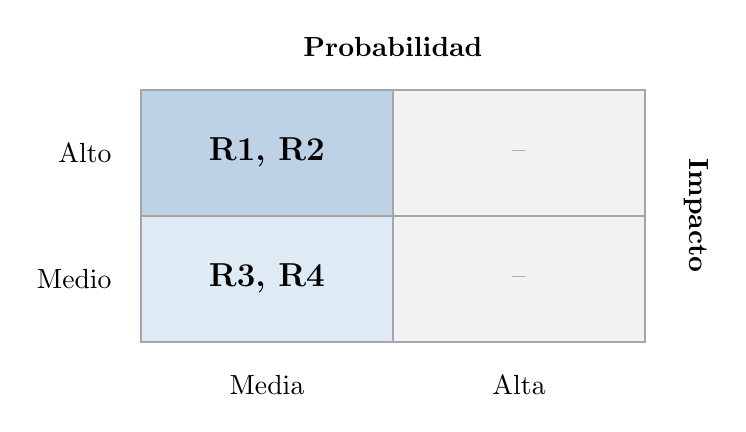
\begin{tikzpicture}
\definecolor{cellhigh}{RGB}{190,210,230}
\definecolor{cellmed}{RGB}{222,234,244}
\definecolor{cellempty}{RGB}{242,242,242}
\fill[cellhigh] (0,1.6) rectangle (3.2,3.2);
\fill[cellempty] (3.2,1.6) rectangle (6.4,3.2);
\fill[cellmed] (0,0) rectangle (3.2,1.6);
\fill[cellempty] (3.2,0) rectangle (6.4,1.6);
\draw[gray!70, line width=0.6pt] (0,0) rectangle (6.4,3.2);
\draw[gray!70, line width=0.6pt] (3.2,0) -- (3.2,3.2);
\draw[gray!70, line width=0.6pt] (0,1.6) -- (6.4,1.6);
\node[font=\large\bfseries] at (1.6,2.4) {R1,~R2};
\node[font=\large\bfseries] at (1.6,0.8) {R3,~R4};
\node[font=\normalsize, gray] at (4.8,2.4) {--};
\node[font=\normalsize, gray] at (4.8,0.8) {--};
\node[font=\normalsize, anchor=east] at (-0.25,2.4) {Alto};
\node[font=\normalsize, anchor=east] at (-0.25,0.8) {Medio};
\node[font=\normalsize, anchor=north] at (1.6,-0.3) {Media};
\node[font=\normalsize, anchor=north] at (4.8,-0.3) {Alta};
\node[font=\normalsize\bfseries] at (3.2,3.75) {Probabilidad};
\node[font=\normalsize\bfseries, rotate=-90] at (7.05,1.6) {Impacto};
\end{tikzpicture}%
}
\caption{Matriz probabilidad--impacto con ubicación de los riesgos identificados. Elaboración propia.}\label{fig:matriz-pi}
\end{figure}

La suma de impactos en el peor caso (+44\,h) es inferior a la holgura disponible (aproximadamente 60\,h), lo que garantiza la viabilidad temporal incluso activando todos los planes simultáneamente~\cite{pmbok}. Esto no significa que los riesgos sean despreciables, sino que la planificación los ha absorbido de forma explícita. La Figura~\ref{fig:holgura} visualiza esta relación.

\begin{figure}[H]
\centering
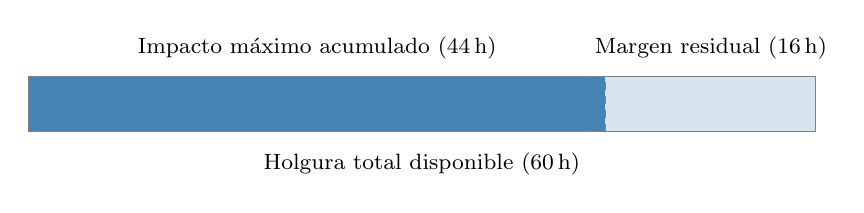
\begin{tikzpicture}
\definecolor{barblue}{RGB}{70,130,180}
\definecolor{barlight}{RGB}{215,228,240}
\fill[barlight] (0,0) rectangle (10,0.7);
\fill[barblue] (0,0) rectangle (7.33,0.7);
\draw[gray] (0,0) rectangle (10,0.7);
\draw[gray, densely dashed] (7.33,0) -- (7.33,0.7);
\node[font=\footnotesize, anchor=south] at (3.67,0.8) {Impacto máximo acumulado (44\,h)};
\node[font=\footnotesize, anchor=south] at (8.67,0.8) {Margen residual (16\,h)};
\node[font=\footnotesize, anchor=north] at (5,-0.15) {Holgura total disponible (60\,h)};
\end{tikzpicture}
\caption{Comparación entre la holgura disponible y el impacto acumulado de riesgos en el peor caso. Elaboración propia.}\label{fig:holgura}
\end{figure}

\subsection{Seguimiento y control}

El seguimiento combina dos mecanismos complementarios. Por un lado, la documentación continua (TG.2), que se actualiza tras cada tarea técnica con README, decisiones de diseño y resultados. Por otro, las reuniones quincenales de seguimiento (TG.1), donde contrasto el avance real frente al plan~\cite{gep23}.

El instrumento central de registro es una hoja de seguimiento semanal mantenida en el repositorio del proyecto. En ella anoto, para cada tarea del WBS, las horas planificadas acumuladas y las horas reales ejecutadas hasta la fecha, junto con el porcentaje de avance estimado y cualquier incidencia relevante. Esta comparación sistemática entre lo previsto y lo ejecutado se inspira en el concepto de valor ganado (\textit{Earned Value}) descrito en el PMBOK~\cite{pmbok}, adaptado a la escala de un TFG individual sin la formalidad completa de un cuadro de mando corporativo.

Como indicador cuantitativo, monitorizo semanalmente el porcentaje de horas ejecutadas respecto al acumulado previsto, usando el Gantt como línea base. Si la desviación supera el 15\,\%, se convoca reunión extraordinaria para decidir replanificación o activación de planes alternativos. Este umbral está pensado para detectar desviaciones antes de que comprometan hitos posteriores del camino crítico.

Una tarea se cierra formalmente cuando su evidencia está en el repositorio y cumple el criterio de aceptación del WBS, con trazabilidad completa a través de los commits en Git y registro de decisiones en \texttt{CHANGELOG.md}. Además, tras cada hito H1--H8 se realiza una verificación formal de cumplimiento cuyo resultado queda registrado en el repositorio junto con la evidencia del entregable correspondiente. La combinación de la hoja de seguimiento, las reuniones quincenales, la documentación continua y la verificación por hitos garantiza que ninguna desviación significativa pase inadvertida durante más de dos semanas~\cite{gep23}.

\subsection{Análisis crítico y coherencia de la planificación}

Toda planificación es, por definición, una hipótesis sobre el futuro, y conviene ser honesto con sus limitaciones antes de defenderla. En mi caso, he intentado construir un plan que sea a la vez ambicioso en alcance y prudente en márgenes, pero hay factores que escapan a mi control y que podrían alterar la ejecución prevista.

La principal fuente de incertidumbre es la dependencia de las colas GPU de MareNostrum~5, un recurso compartido cuya disponibilidad efectiva no puedo garantizar. A esto se suma que la cadena F4--F5--F6 es estrictamente secuencial y acumula 172 horas, de modo que cualquier retraso en una fase se propaga íntegramente a las siguientes. Si el desfase acumulado superase las dos semanas, la decisión más probable sería prescindir de Política~C y presentar únicamente A y~B, lo que reduciría el alcance pero preservaría la contribución central del TFG. Las estimaciones de las tareas experimentales (especialmente T5.5 y T6.5) llevan además un componente de incertidumbre mayor que las de infraestructura o documentación, porque dependen de la convergencia del entrenamiento y de la curva de aprendizaje con herramientas que aún no he usado de forma intensiva. Precisamente por eso he incorporado márgenes internos superiores al 20\,\% en esas tareas y he reservado tres semanas de holgura global (60\,h), dimensionadas para absorber el peor caso acumulado de los cuatro riesgos (+44\,h)~\cite{pmbok}.

Con todo, considero la planificación realista y coherente. Las 540\,h encajan con la carga de 15 ECTS más GEP, la dedicación semanal está calibrada con mi disponibilidad real, y la integración entre WBS, Gantt, registro de riesgos y mecanismos de seguimiento cubre las cuatro dimensiones fundamentales del PMBOK (alcance, tiempo, recursos y riesgos) dentro de un sistema de control que se revisa y actualiza semanalmente~\cite{gep23,gpi}.

%%%%%%%%%%%%%%%%%%%%%%%%%%%%%%%%%%%%%%%%%%%%%%%%%%%%%%%%%%%%%%%%%
\section{Presupuesto y sostenibilidad del proyecto}

\subsection{Supuestos económicos y criterios de cálculo}

El presupuesto estima el coste real que tendría el proyecto si fuera ejecutado por un equipo profesional en un contexto de empresa o consultoría tecnológica. Se trata de un presupuesto de coste de oportunidad, no de gasto personal del autor. Los supuestos son los siguientes.

\begin{itemize}[nosep]
\item \textbf{Referencia salarial base.} La Guía del Mercado Laboral 2026 de Hays~\cite{hays2026} de perfiles TIC en Barcelona proporciona los salarios de referencia. Los salarios corresponden a perfiles senior con tres a cinco años de experiencia, coherentes con la especialización técnica requerida por el proyecto.
\item \textbf{Tasa horaria cargada.} Se aplica la fórmula estándar de consultoría tecnológica en España de la siguiente forma:
\[
\text{Tasa cargada} = \frac{\text{Bruto anual}}{1.720}\;\times\;1{,}3\;(\text{SS})\;\times\;2{,}0\;(\text{overhead + margen})
\]
El factor 2,0 recoge gastos de estructura empresarial, beneficios sociales, equipamiento, administración y margen operativo, tal como aplican las empresas de servicios tecnológicos en proyectos de investigación y desarrollo.
\item \textbf{Duración del proyecto.} El proyecto dura 19 semanas, aproximadamente cinco meses efectivos, conforme al WBS de la planificación del proyecto~\cite{gep23e2}.
\item \textbf{Horas totales.} Se presupuestan 540 horas distribuidas en cuatro perfiles: Cap de projecte con 140 horas, Data scientist con 120 horas, ML engineer con 172 horas, y DevOps con 108 horas, sin modificar la distribución por tareas.
\item \textbf{Infraestructura HPC.} Se presupuesta a coste de mercado equivalente al precio on-demand de AWS, dado que el análisis de sostenibilidad económica debe reflejar el coste real del recurso si no hubiera acceso institucional. En la sección de sostenibilidad se distingue entre el coste presupuestado y el coste real para el autor.
\item \textbf{Costes indirectos.} Se estima el 20 por ciento sobre los costes de personal, como estimación estándar de overhead de estructura para proyectos informáticos.
\item \textbf{Contingencia.} Se aplica el 15 por ciento sobre el subtotal directo, dentro del rango recomendado del 10 a 20 por ciento para proyectos informáticos~\cite{gep23}.
\item \textbf{Imprevistos.} Se cuantifica como valor esperado de los riesgos R1 a R4 definidos en la planificación~\cite{gep23e2}, calculado como el producto del impacto económico por la probabilidad.
\end{itemize}

\subsection{Costes de personal (RRHH)}

La Tabla~\ref{tab:costes-rol} muestra los cuatro perfiles del equipo con sus tasas horarias cargadas.

\begin{table}[H]
\centering
\caption{Perfiles del equipo y tasa horaria cargada. Fuente: elaboración propia a partir de~\cite{hays2026}.}
\label{tab:costes-rol}
\footnotesize
\begin{tabular}{l l r r r}
\toprule
\textbf{Perfil (rol)} & \textbf{Equiv.\ Hays 2026 (senior)} & \textbf{Bruto anual (\euro{})} & \textbf{Bruto/h\,+\,SS (\euro{})} & \textbf{Tasa cargada (\euro{}/h)} \\
\midrule
Cap de projecte (CP)   & Project Manager Senior  & 60.000 & 45,35 & 87,00 \\
Data scientist (DS)    & Data Scientist Senior   & 55.000 & 41,57 & 82,00 \\
ML engineer (ML)       & ML / AI Engineer Senior & 65.000 & 49,13 & 98,00 \\
DevOps-HPC (DV)        & DevOps Engineer Senior  & 55.000 & 41,57 & 82,00 \\
\bottomrule
\end{tabular}
\end{table}

\noindent\textit{\scriptsize Tasa cargada = (Bruto anual / 1.720) $\times$ 1,3 (SS empleador) $\times$ 2,0 (factor overhead y margen). Referencia salarial: Hays España 2026~\cite{hays2026}, sección TIC, Barcelona, perfil senior (3--5 años de experiencia). El factor 2,0 es coherente con el modelo de facturación de proyectos de I+D en empresas de servicios tecnológicos.}

\noindent Los perfiles, la distribución de horas por tarea y los totales por rol coinciden con la planificación del proyecto~\cite{gep23e2}.

\subsection{Costes de personal por actividad (CPA)}

Cada tarea del WBS tiene un coste económico asociado, calculado como el producto de las horas estimadas por la tasa horaria cargada del perfil responsable:
\[
C_{\text{tarea}_i} = h_{\text{tarea}_i} \times \text{Tasa}_{\text{perfil}}
\]
Esta vinculación directa garantiza la trazabilidad entre la planificación temporal (diagrama de Gantt), la asignación de recursos humanos y la estimación económica del proyecto.

La Tabla~\ref{tab:cpa} desglosa el coste de personal por cada tarea del WBS, con subtotales por fase, usando las tasas cargadas de la Tabla~\ref{tab:costes-rol}. En las tareas con doble rol (marcadas con~$\dagger$), el coste se imputa al rol predominante. La tarea TG.2 (documentación continua) distribuye sus 30\,h entre los cuatro perfiles tal como se definió en la planificación~\cite{gep23e2}.

{\scriptsize
\setlength{\tabcolsep}{3pt}
\renewcommand{\arraystretch}{0.88}
\begin{tabularx}{\textwidth}{>{\ttfamily}l >{\raggedright\arraybackslash}X r l r r}
\caption{Costes por actividad del WBS (CPA). Fuente: elaboración propia.}\label{tab:cpa}\\
\toprule
\textbf{Cód.} & \textbf{Tarea} & \textbf{h} & \textbf{Rol} & \textbf{\euro{}/h} & \textbf{Coste (\euro{})} \\
\midrule
\endfirsthead
\multicolumn{6}{l}{\textit{(continuación de la Tabla~\ref{tab:cpa})}} \\
\toprule
\textbf{Cód.} & \textbf{Tarea} & \textbf{h} & \textbf{Rol} & \textbf{\euro{}/h} & \textbf{Coste (\euro{})} \\
\midrule
\endhead
\midrule
\multicolumn{6}{r}{\textit{Continúa en la página siguiente}} \\
\endfoot
\bottomrule
\endlastfoot
T1.1 & Acceso y cuenta BSC & 4 & DV & 82,00 & 328,00 \\
T1.2 & Entorno y scripts SLURM base & 10 & DV & 82,00 & 820,00 \\
T1.3 & Instalar vLLM y dependencias & 12 & DV & 82,00 & 984,00 \\
T1.4 & Preparar teacher y cachés$\,^\dagger$ & 10 & ML & 98,00 & 980,00 \\
T1.5 & Desplegar API teacher y healthchecks & 12 & DV & 82,00 & 984,00 \\
\multicolumn{2}{r}{\textit{Subtotal F1}} & \textit{48} & & & \textit{4.096,00} \\
\addlinespace[1.5pt]
T2.1 & Definir esquema req-resp y logs$\,^\dagger$ & 6 & DS & 82,00 & 492,00 \\
T2.2 & Impl.\ cliente benchmark y conc. & 12 & ML & 98,00 & 1.176,00 \\
T2.3 & Muestreador de prompts y norm. & 6 & ML & 98,00 & 588,00 \\
T2.4 & Validación 10\,000 peticiones & 8 & ML & 98,00 & 784,00 \\
\multicolumn{2}{r}{\textit{Subtotal F2}} & \textit{32} & & & \textit{3.040,00} \\
\addlinespace[1.5pt]
T3.1 & Instrumentación latencia y tokens$\,^\dagger$ & 8 & ML & 98,00 & 784,00 \\
T3.2 & Experimentos de carga (sweep) & 14 & ML & 98,00 & 1.372,00 \\
T3.3 & Registro memoria y uso GPU & 6 & DV & 82,00 & 492,00 \\
T3.4 & Agregación p50/p95 y tablas & 8 & DS & 82,00 & 656,00 \\
\multicolumn{2}{r}{\textit{Subtotal F3}} & \textit{36} & & & \textit{3.304,00} \\
\addlinespace[1.5pt]
T4.1 & Preparar eval.\ GSM8K y MATH & 8 & DS & 82,00 & 656,00 \\
T4.2 & Ejecutar evaluación teacher & 14 & ML & 98,00 & 1.372,00 \\
T4.3 & Análisis errores y baseline calidad & 12 & DS & 82,00 & 984,00 \\
\multicolumn{2}{r}{\textit{Subtotal F4}} & \textit{34} & & & \textit{3.012,00} \\
\addlinespace[1.5pt]
T5.1 & Selección student candidato & 6 & DS & 82,00 & 492,00 \\
T5.2 & Baseline student (mismo prot.) & 12 & ML & 98,00 & 1.176,00 \\
T5.3 & Decisión viabilidad destilación$\,^\dagger$ & 6 & DS & 82,00 & 492,00 \\
T5.4 & Preparar pipeline destilación & 12 & ML & 98,00 & 1.176,00 \\
T5.5 & Ejecutar destilación o alternativa & 22 & ML & 98,00 & 2.156,00 \\
T5.6 & Evaluar student destilado$\,^\dagger$ & 12 & DS & 82,00 & 984,00 \\
\multicolumn{2}{r}{\textit{Subtotal F5}} & \textit{70} & & & \textit{6.476,00} \\
\addlinespace[1.5pt]
T6.1 & Definir criterio quality gate & 6 & DS & 82,00 & 492,00 \\
T6.2 & Impl.\ Política B (cascada forc.) & 14 & ML & 98,00 & 1.372,00 \\
T6.3 & Evaluar Política B vs A$\,^\dagger$ & 12 & DS & 82,00 & 984,00 \\
T6.4 & Preparar features y dataset pred.$\,^\dagger$ & 10 & DS & 82,00 & 820,00 \\
T6.5 & Entrenar predictor (Política C) & 16 & ML & 98,00 & 1.568,00 \\
T6.6 & Evaluar Política C vs A y B$\,^\dagger$ & 10 & DS & 82,00 & 820,00 \\
\multicolumn{2}{r}{\textit{Subtotal F6}} & \textit{68} & & & \textit{6.056,00} \\
\addlinespace[1.5pt]
T7.1 & Esqueleto memoria y reprod. & 8 & CP & 87,00 & 696,00 \\
T7.2 & Redacción metodología y entorno & 12 & DV & 82,00 & 984,00 \\
T7.3 & Redacción resultados teacher/stud. & 16 & DS & 82,00 & 1.312,00 \\
T7.4 & Redacción routing y discusión & 16 & ML & 98,00 & 1.568,00 \\
T7.5 & Presentación y guion defensa & 10 & CP & 87,00 & 870,00 \\
T7.6 & Revisión final y entrega & 10 & CP & 87,00 & 870,00 \\
\multicolumn{2}{r}{\textit{Subtotal F7}} & \textit{72} & & & \textit{6.300,00} \\
\addlinespace[1.5pt]
TG.1 & Reuniones de seguimiento & 12 & CP & 87,00 & 1.044,00 \\
TG.2 & Doc.\ continua (coord.\ y registro) & 10 & CP & 87,00 & 870,00 \\
TG.2 & Doc.\ continua (experimentos) & 8 & DS & 82,00 & 656,00 \\
TG.2 & Doc.\ continua (código y decisiones) & 8 & ML & 98,00 & 784,00 \\
TG.2 & Doc.\ continua (infra.\ y entorno) & 4 & DV & 82,00 & 328,00 \\
TG.3 & Gestión repositorio y versionado & 48 & DV & 82,00 & 3.936,00 \\
\multicolumn{2}{r}{\textit{Subtotal TG}} & \textit{90} & & & \textit{7.618,00} \\
\addlinespace[1.5pt]
GP & Gestión del proyecto & 90 & CP & 87,00 & 7.830,00 \\
\midrule
\multicolumn{2}{r}{\textbf{TOTAL CPA}} & \textbf{540} & & & \textbf{47.732,00} \\
\end{tabularx}
}

\noindent\textit{\scriptsize $\dagger$\,Tarea con doble rol en la planificación; coste imputado al rol predominante. Verificación por rol: CP\,140\,h\,$\times$\,87,00\,=\,12.180,00; DS\,120\,h\,$\times$\,82,00\,=\,9.840,00; ML\,172\,h\,$\times$\,98,00\,=\,16.856,00; DV\,108\,h\,$\times$\,82,00\,=\,8.856,00. Suma\,=\,47.732,00\,\euro{}.}

\subsection{Costes de infraestructura}

Aunque el acceso a MareNostrum~5 está concedido por el BSC sin coste directo, el presupuesto refleja el coste equivalente de mercado para garantizar la validez del análisis económico.

Las horas de GPU se derivan del diseño experimental. Se contemplan entre tres y cinco configuraciones de modelo evaluadas sobre GSM8K y MATH, con dos a tres repeticiones por configuración. El proyecto se centra en inferencia y destilación supervisada, no en preentrenamiento desde cero, por lo que la demanda de GPU es considerablemente inferior a la de proyectos de entrenamiento completo. Se estiman 75 GPU-h planificadas más un 33 por ciento de reserva, lo que da un total de 100 GPU-h presupuestadas.

\begin{table}[H]
\centering
\caption{Costes de infraestructura. Fuente: elaboración propia a partir de~\cite{lambda2026,aws2026}.}
\label{tab:infraestructura}
\footnotesize
\begin{tabular}{l l r r r}
\toprule
\textbf{Recurso} & \textbf{Justificación} & \textbf{Cantidad} & \textbf{\euro{}/unidad} & \textbf{Coste (\euro{})} \\
\midrule
GPU H100 on-demand (AWS \texttt{p5.xlarge})  & 100\,GPU-h\,$\times$\,10,98\,\euro{}/h~\cite{aws2026} & 100\,h & 10,98 & 1.098,00 \\
Almacenamiento NFS (500\,GB, 5 meses)        & datasets, checkpoints, logs    & 5\,meses & 80,00 & 400,00 \\
Transferencia de red y egress                & descarga de modelos, backups   & estimación & -- & 150,00 \\
Monitorización y logging (cloud)             & métricas, alertas, dashboards  & 5\,meses & 40,00 & 200,00 \\
Cuota BSC imputada (simbólica)               & fracción cuota grupo inv.      & 5\,meses & 30,00 & 150,00 \\
\midrule
\textbf{Total infraestructura} & & & & \textbf{1.998,00} \\
\bottomrule
\end{tabular}
\end{table}

\noindent\textit{\scriptsize La GPU H100 se presupuesta a precio on-demand de AWS (instancia \texttt{p5.xlarge}, us-east-1)~\cite{aws2026}. Se estiman 100\,GPU-h: 75\,h planificadas más un 33\,\% de reserva para fallos, reruns y tuning. El almacenamiento cubre: dataset GSM8K/MATH ($\approx$\,100\,MB), checkpoints de modelos 7B--14B ($\approx$\,30\,GB), logs experimentales y versiones del código. La cuota BSC es una imputación simbólica que refleja el uso proporcional del acceso institucional.}

\subsection{Costes de software y herramientas}

Todo el software utilizado es de naturaleza intrínsecamente gratuita. El stack técnico se distribuye bajo licencias de código abierto como Apache 2.0 y BSD, y las herramientas complementarias son igualmente libres u open source. El coste de software se declara como cero euros, tal como recoge la Tabla~\ref{tab:software}.

\begin{table}[H]
\centering
\caption{Costes de software y herramientas. Fuente: elaboración propia.}
\label{tab:software}
\footnotesize
\begin{tabular}{l r r}
\toprule
\textbf{Recurso} & \textbf{Coste/mes (\euro{})} & \textbf{Coste final (\euro{})} \\
\midrule
vLLM, PyTorch, Python, NumPy, Transformers (HuggingFace) & 0 & 0,00 \\
Git, GitHub (plan Free / Student Developer Pack)         & 0 & 0,00 \\
VS~Code, Linux, Slurm (software del BSC)                 & 0 & 0,00 \\
Overleaf (plan Free, usuario único)                      & 0 & 0,00 \\
\midrule
\textbf{Total software} & & \textbf{0,00} \\
\bottomrule
\end{tabular}
\end{table}

\noindent\textit{\scriptsize Todo el software del proyecto tiene coste cero. El stack técnico (vLLM, PyTorch, Python, NumPy, Transformers) es open source bajo licencias Apache 2.0 y BSD. Git es open source y GitHub ofrece planes gratuitos. VS~Code es software libre y las herramientas de sistema del BSC (Linux, Slurm) son igualmente open source. Overleaf ofrece un plan gratuito suficiente para este proyecto. Ningún componente requiere pago por licencias comerciales.}

\subsection{Costes indirectos y estructurales}

Los costes indirectos incluyen los gastos del entorno de trabajo y un overhead de estructura empresarial del 20 por ciento sobre los costes de personal. Este overhead recoge administración, coordinación, infraestructura de oficina y soporte organizativo, y es un valor conservador habitual en proyectos tecnológicos de pequeña escala~\cite{pmbok}.

\begin{table}[H]
\centering
\caption{Costes estructurales directos. Fuente: elaboración propia.}
\label{tab:estructurales}
\footnotesize
\begin{tabular}{l l r}
\toprule
\textbf{Concepto} & \textbf{Cálculo} & \textbf{Subtotal (\euro{})} \\
\midrule
Espacio de trabajo (home office)    & 5 meses $\times$ 400\,\euro{}/mes               & 2.000,00 \\
Internet (fibra doméstica)          & 5 meses $\times$ 15\,\euro{}/mes                & 75,00  \\
Teléfono / comunicaciones           & 5 meses $\times$ 10\,\euro{}/mes                & 50,00  \\
Material fungible                   & estimación global                               & 50,00  \\
Impresión y encuadernación TFG      & 2 copias $\times$ 15\,\euro{}                   & 30,00  \\
Desplazamientos                     & trabajo íntegramente remoto (BSC vía SSH)       & 0,00   \\
\midrule
\textbf{Subtotal estructurales directos} & & \textbf{2.205,00} \\
\addlinespace[4pt]
Overhead de estructura empresarial  & 20\,\% $\times$ CPA (47.732,00\,\euro{})        & 9.546,40 \\
\midrule
\textbf{Total costes indirectos y estructurales} & & \textbf{11.751,40} \\
\bottomrule
\end{tabular}
\end{table}

\noindent\textit{\scriptsize Overhead del 20 por ciento: estimación conservadora para I+D con equipo reducido. En proyectos de mayor escala puede alcanzar entre el 30 y el 40 por ciento.}

\subsection{Amortización de hardware}

Los equipos de desarrollo se amortizan linealmente, imputando únicamente la fracción proporcional a los cinco meses del proyecto según la siguiente fórmula:

\[
\text{Coste amortizado} = \frac{\text{Precio de adquisición}}{\text{Vida útil en meses}} \times \text{Meses imputados}
\]

\begin{table}[H]
\centering
\caption{Amortización de hardware. Fuente: elaboración propia.}
\label{tab:hardware}
\footnotesize
\begin{tabular}{l r r r r}
\toprule
\textbf{Dispositivo} & \textbf{Precio (\euro{})} & \textbf{Vida útil (meses)} & \textbf{Meses imput.} & \textbf{Coste amort.\ (\euro{})} \\
\midrule
Portátil de desarrollo & 1.200,00 & 48 & 5 & 125,00 \\
Monitor externo (24'') & 200,00   & 60 & 5 & 16,67  \\
\midrule
\textbf{Total hardware} & & & & \textbf{141,67} \\
\bottomrule
\end{tabular}
\end{table}

\noindent\textit{\scriptsize Vida útil del portátil: cuatro años, equivalentes a 48 meses, estándar fiscal para equipos informáticos en España. Monitor: cinco años, equivalentes a 60 meses. Los precios corresponden a precio de venta al público de referencia en el momento de la adquisición.}

\subsection{Imprevistos asociados a riesgos}

Los riesgos R1 a R4 de la planificación~\cite{gep23e2} se cuantifican como el producto de su impacto económico por su probabilidad de ocurrencia. El impacto se valora a la tasa del ML engineer de 98 euros por hora, por ser el perfil más afectado, y la probabilidad Media se fija en 0,4. La Tabla~\ref{tab:imprevistos} recoge el coste esperado resultante.

\begin{table}[H]
\centering
\caption{Imprevistos asociados a riesgos. Fuente: elaboración propia a partir de la planificación del proyecto~\cite{gep23e2}.}
\label{tab:imprevistos}
\footnotesize
\begin{tabular}{l l r r r r}
\toprule
\textbf{Riesgo} & \textbf{Rol} & \textbf{+h} & \textbf{Impacto (\euro{})} & \textbf{Prob.} & \textbf{Esperado (\euro{})} \\
\midrule
R1. Colas GPU saturadas     & ML & 20 & 1.960,00 & 0,4 & 784,00  \\
R2. Destilación inviable    & ML & 6  & 588,00   & 0,4 & 235,20  \\
R3. Predictor no generaliza & ML & 10 & 980,00   & 0,4 & 392,00  \\
R4. Latencia routing        & ML & 8  & 784,00   & 0,4 & 313,60  \\
\midrule
\textbf{Total} & & \textbf{44} & \textbf{4.312,00} & & \textbf{1.724,80} \\
\bottomrule
\end{tabular}
\end{table}

\noindent\textit{\scriptsize Impacto igual a horas extra multiplicadas por 98 euros por hora, que es la tasa cargada para ML engineer senior. Coste esperado igual a impacto multiplicado por probabilidad.}

\subsection{Coste total estimado del proyecto}

El presupuesto incluye una reserva global de contingencia del 15 por ciento sobre el subtotal directo, práctica habitual en proyectos de ingeniería informática para absorber desviaciones imprevistas no cubiertas por los riesgos identificados~\cite{pmbok}. Su cálculo es:
\[
\text{Contingencia} = 0{,}15 \times \text{Subtotal directo} = 0{,}15 \times 61.623{,}07 = 9.243{,}46\;\text{\euro{}}
\]
Este porcentaje se sitúa dentro del rango del 10 al 20 por ciento recomendado para proyectos de I+D de pequeña escala.

\begin{table}[H]
\centering
\caption{Coste total estimado del proyecto. Fuente: elaboración propia.}
\label{tab:total}
\footnotesize
\begin{tabular}{l r}
\toprule
\textbf{Partida} & \textbf{Importe (\euro{})} \\
\midrule
Costes de personal por actividad (CPA)  & 47.732,00 \\
Costes de infraestructura               & 1.998,00  \\
Costes de software y herramientas       & 0,00      \\
Amortización de hardware                & 141,67    \\
Costes indirectos y estructurales       & 11.751,40 \\
\cmidrule{2-2}
Subtotal directo                        & 61.623,07 \\
Contingencia (15\,\%)                   & 9.243,46  \\
Imprevistos (coste esperado)            & 1.724,80  \\
\midrule
\textbf{TOTAL PROYECTO}                 & \textbf{72.591,33} \\
\bottomrule
\end{tabular}
\end{table}

\begin{figure}[H]
\centering
\begin{tikzpicture}
\pie[text=legend, radius=2.15, color={blue!35,orange!45,gray!35}]{65.8/RRHH,2.8/Infraestructura,31.4/Costes operativos e indirectos}
\end{tikzpicture}
\caption{Distribución porcentual del presupuesto total por partidas principales. Fuente: elaboración propia.}
\label{fig:distribucion-presupuesto}
\end{figure}

\noindent El presupuesto es coherente con las 540 horas de la planificación~\cite{gep23e2}. La partida de personal representa el 66 por ciento del total, los costes de software son cero al emplear exclusivamente software libre, y la infraestructura supone el 3 por ciento, reflejando el coste de mercado de GPUs H100 en cloud. El coste total de 72.591 euros se sitúa dentro del rango razonable para proyectos de investigación aplicada en inteligencia artificial de pequeña escala.

\subsection{Control económico y seguimiento del presupuesto}

El seguimiento se realiza de forma semanal y al cierre de cada fase, registrando horas reales por tarea y rol, gastos de infraestructura y horas de GPU por experimento mediante JobID SLURM.

Los indicadores cuantitativos de control son los siguientes. La desviación absoluta y porcentual por tarea permiten detectar sobrecostes puntuales:
\[
\Delta C_{\text{tarea}} = C_{\text{real}} - C_{\text{plan}} \qquad
\Delta C\% = \frac{C_{\text{real}} - C_{\text{plan}}}{C_{\text{plan}}} \times 100
\]
La desviación de horas por rol y de horas de GPU permiten controlar el consumo de recursos:
\[
\Delta h_{\text{rol}} = h_{\text{real,rol}} - h_{\text{plan,rol}} \qquad
\Delta \text{GPU} = \text{GPU-h}_{\text{real}} - \text{GPU-h}_{\text{plan}}
\]
Adicionalmente se calcula el índice de rendimiento de costes (CPI) mediante la técnica del valor ganado (Earned Value Management), que proporciona una medida normalizada de la eficiencia económica del proyecto:
\[
\text{CPI} = \frac{\text{EV}}{\text{AC}}
\]
donde EV (Earned Value) es el valor del trabajo completado según el presupuesto planificado y AC (Actual Cost) es el coste real incurrido. Un CPI superior a 1 indica que el proyecto se ejecuta por debajo del presupuesto, mientras que un CPI inferior a 1 señala un sobrecoste que requiere acciones correctivas como la repriorización de tareas, la reasignación de recursos o el ajuste de alcance. El coste acumulado del proyecto se compara periódicamente con la curva de gasto planificada al cierre de cada fase, permitiendo detectar desviaciones de forma temprana.

Los umbrales y acciones correctivas se establecen de la siguiente forma:
\begin{itemize}[nosep]
\item Si la desviación de coste supera el 15 por ciento en una fase del camino crítico, de la F1 a la F6, se convoca una reunión extraordinaria con posible replanificación o recorte de alcance priorizando las Políticas A y B.
\item Si la desviación de coste supera el 25 por ciento en cualquier fase, se congelan las configuraciones experimentales y se reducen las repeticiones al mínimo, de tres a dos.
\item Si la desviación en GPU supera 50 horas antes de la semana 10, se activa el plan de contingencia R1 con jobs nocturnos, reducción de repeticiones y limitación de sweeps.
\item Si la desviación de horas por rol supera el 20 por ciento al cierre de fase, se rebalancea el esfuerzo en las fases siguientes.
\end{itemize}

\noindent La hoja de seguimiento semanal, las reuniones quincenales TG.1 y la verificación por hitos H1 a H8 garantizan que ninguna desviación significativa pase inadvertida más de dos semanas.

\subsection{Marco general de la sostenibilidad}

A lo largo de mis estudios en el Grado de Ingeniería Informática en la FIB he podido profundizar en los aspectos clave de la sostenibilidad a través de diversas asignaturas, lo que me ha llevado a reconocer su importancia al desarrollar este TFG. Tras completar la encuesta del proyecto de investigación EDINSOST2-ODS sobre desarrollo sostenible, se ha realizado una autoevaluación del impacto del proyecto en las tres dimensiones de sostenibilidad.

La sostenibilidad, entendida desde una perspectiva integral que abarca las dimensiones económica, social y ambiental, es un factor relevante en cualquier proyecto tecnológico. En el contexto de proyectos que hacen uso intensivo de infraestructura de computación de altas prestaciones y modelos de lenguaje de gran tamaño, estas dimensiones están estrechamente interrelacionadas dado que la eficiencia computacional reduce simultáneamente costes, consumo energético y barreras de acceso. Un análisis adecuado permite no solo reducir el impacto inmediato sino también aportar soluciones sostenibles aplicables a proyectos futuros.

Me comprometo a registrar y publicar el consumo energético real de cada experimento comparándolo con las estimaciones de este documento, y a dedicar una sección de la memoria del TFG al balance neto de sostenibilidad del sistema de cascada.

\subsection{Dimensión económica}

Después de revisar el presupuesto del proyecto, considero que es apropiado teniendo en cuenta los beneficios que puede aportar. El coste total estimado asciende a 72.591 euros como coste de oportunidad, mientras que el gasto real para el autor es prácticamente cero dado que la infraestructura está cedida por el BSC y el software es intrínsecamente gratuito. Este proyecto tiene el potencial de ahorrar una cantidad significativa de recursos computacionales a las organizaciones que adopten el sistema de cascada, lo que se traduce en un ahorro de costes a largo plazo.

Desde el punto de vista de la viabilidad en producción, un sistema de cascada que derive el 60 por ciento de las peticiones al student puede reducir las GPU horas anuales aproximadamente un 30 por ciento. La Tabla~\ref{tab:ahorro-cascada} estima el ahorro anual proyectado según proveedor cloud~\cite{lambda2026,aws2026}.

\begin{table}[H]
\centering
\caption{Estimación de ahorro anual con sistema de cascada según proveedor cloud. Fuente: elaboración propia a partir de~\cite{lambda2026,aws2026}.}
\label{tab:ahorro-cascada}
\footnotesize
\begin{tabular}{l r r r r}
\toprule
\textbf{Proveedor} & \textbf{\euro{}/GPU-h} & \textbf{GPU-h/año (solo teacher)} & \textbf{Ahorro 30\,\%} & \textbf{Ahorro anual (\euro{})} \\
\midrule
Lambda Labs  & 2,49  & 8.760 & 2.628\,h & 6.544 \\
AWS (p5.xlarge) & 10,98 & 8.760 & 2.628\,h & 28.855 \\
\bottomrule
\end{tabular}
\end{table}

\noindent\textit{\scriptsize Se asume un despliegue continuo de una GPU H100 durante un año completo, equivalente a 8.760 GPU horas. El ahorro del 30 por ciento corresponde al escenario en que el sistema de cascada redirija el 60 por ciento de las peticiones al student con una tasa de fallback inferior al 40 por ciento.}

Esta viabilidad hace el proyecto relevante para organizaciones con recursos limitados. La vida útil de los resultados se estima entre dos y tres años, aunque los principios de diseño del routing y la destilación seguirán siendo aplicables más allá de ese horizonte.

\subsection{Dimensión ambiental}

El impacto ambiental se concentra en el consumo energético de las GPUs H100 durante las fases experimentales. La Tabla~\ref{tab:consumo-fase} desglosa la estimación por fase, asumiendo 375 watts por GPU y un factor de emisión de 0,20 kg CO\textsubscript{2}/kWh~\cite{ree2024}.

\begin{table}[H]
\centering
\caption{Estimación de consumo energético y emisiones por fase experimental. Fuente: elaboración propia a partir de~\cite{ree2024}.}
\label{tab:consumo-fase}
\footnotesize
\begin{tabular}{l r r r}
\toprule
\textbf{Fase experimental} & \textbf{GPU-h estimadas} & \textbf{Consumo (kWh)} & \textbf{CO\textsubscript{2}eq (kg)} \\
\midrule
Caracterización teacher (F2 a F4)         & 15 & 5,63  & 1,13 \\
Destilación del student (F5)              & 30 & 11,25 & 2,25 \\
Evaluación políticas routing (F6)         & 20 & 7,50  & 1,50 \\
Reruns exploratorios y ajustes (F3 a F5)  & 10 & 3,75  & 0,75 \\
\midrule
\textbf{Total planificado}                & \textbf{75} & \textbf{28,13} & \textbf{5,63} \\
\addlinespace[2pt]
Reserva del 33 por ciento                & 25 & 9,38  & 1,88 \\
\midrule
\textbf{Total presupuestado}              & \textbf{100} & \textbf{37,50} & \textbf{7,50} \\
\bottomrule
\end{tabular}
\end{table}

\noindent\textit{\scriptsize Consumo calculado como GPU-h multiplicadas por 0,375 kW. Emisiones calculadas como kWh multiplicados por 0,20 kgCO\textsubscript{2}/kWh, que es el factor de emisión medio del mix eléctrico español en 2024~\cite{ree2024}. La reserva del 33 por ciento cubre fallos de jobs, reruns y ajustes de configuración.}

El consumo directo planificado ronda los 28 kWh (5,6 kg CO\textsubscript{2}eq), y con la reserva asciende a 37,5 kWh (7,5 kg CO\textsubscript{2}eq). MareNostrum 5 ofrece ventajas ambientales frente a centros de datos comerciales gracias a su eficiencia energética~\cite{mn5}.

El argumento ambiental central del proyecto es que un modelo destilado de siete mil millones de parámetros requiere significativamente menos cómputo por token que el teacher de 14 mil millones, lo que reduce directamente el consumo energético en despliegues a gran escala. Entornos como MareNostrum 5 amplifican esta ventaja gracias a sus sistemas de refrigeración optimizados y economías de escala.

En el peor caso, si todas las consultas pasan por el student sin resolverse antes de redirigirse al teacher, el coste energético por petición sería un 50 por ciento superior al del teacher solo. La Política C mitiga este riesgo con un umbral de confianza que deriva directamente al teacher las peticiones difíciles, y si la tasa de fallback supera el 70 por ciento el sistema revierte automáticamente a servir solo con el teacher. El riesgo de efecto rebote se analizará explícitamente en la memoria del TFG.

A nivel global, el sector de las Tecnologías de la Información y Comunicación representa entre el 2,5 y el 3 por ciento de las emisiones globales de gases de efecto invernadero, con una proyección de aumento para las próximas décadas. En este contexto, proyectos como este que buscan reducir el coste computacional de la inferencia de modelos de lenguaje contribuyen de forma directa a mitigar el impacto ambiental creciente de la inteligencia artificial. Considero que la huella de carbono del proyecto es reducida y proporcionada a los beneficios esperados, y que los resultados obtenidos pueden contribuir a que futuros despliegues de modelos de lenguaje sean más eficientes energéticamente.

Durante la ejecución, el consumo energético de cada job se registrará mediante sacct con el campo ConsumedEnergy, almacenando los resultados en energy\_log.csv. Los valores estimados se contrastarán con las medidas reales y se reportarán en la memoria final.

\subsection{Dimensión social}

Realizar este proyecto en el BSC me ha permitido aprender a gestionar proyectos de investigación aplicada en un entorno de supercomputación real, trabajando con tecnologías punteras como la destilación del conocimiento, la inferencia eficiente de modelos de lenguaje y la orquestación de recursos HPC. Esta experiencia me ha proporcionado una comprensión profunda de cómo optimizar el despliegue de modelos de inteligencia artificial para hacerlo más accesible y eficiente.

El proyecto tiene un impacto social positivo al contribuir a democratizar el acceso a modelos lingüísticos avanzados. La inferencia con modelos de gran tamaño exige GPUs costosas que solo organizaciones con presupuestos elevados pueden permitirse en producción continua. Al reducir los recursos computacionales necesarios mediante destilación y routing inteligente, se amplía el abanico de organizaciones beneficiarias a centros de investigación públicos, universidades y startups con recursos limitados. De manera análoga a cómo la automatización de procesos reduce tiempos de respuesta y mejora la experiencia de los usuarios finales, un sistema de cascada eficiente permite ofrecer servicios de inteligencia artificial de alta calidad a un coste operativo significativamente menor, beneficiando directamente a las organizaciones que lo adopten. La publicación abierta del código, los scripts de evaluación y la documentación del pipeline refuerzan esta transferencia de conocimiento hacia la comunidad investigadora.

A nivel personal, el TFG me ha permitido adquirir competencias en computación de altas prestaciones, reproducibilidad experimental, gestión de proyectos con infraestructura compartida y optimización de modelos de lenguaje. Estas son habilidades con alta demanda en el mercado laboral actual del sector de machine learning e inteligencia artificial, y considero que la formación práctica obtenida durante este proyecto complementa de forma significativa los conocimientos teóricos adquiridos durante el Grado.

Entre los riesgos sociales se identifican el efecto rebote por reducción del coste por petición, la posible amplificación de sesgos del teacher en el student, y la dependencia de infraestructuras de computación de altas prestaciones concentradas en pocas instituciones. Para mitigarlos, el sistema se evaluará con benchmarks objetivos y reproducibles definidos en el alcance, y el pipeline se publicará con sus limitaciones explicitadas. El proyecto no trabaja con datos personales ni toma decisiones automatizadas sobre individuos.

\subsection{Autoevaluación de sostenibilidad}

Tras realizar el análisis de las tres dimensiones, valoro positivamente el ejercicio de reflexión que ha supuesto elaborar este informe de sostenibilidad. Me ha permitido tomar conciencia de que las decisiones técnicas adoptadas durante la planificación del proyecto, como priorizar la destilación del conocimiento frente al uso directo de modelos de gran tamaño o comprometerse a publicar el código de forma abierta, tendrán consecuencias directas sobre la eficiencia económica, el consumo energético y la accesibilidad social de los resultados. Identifico como fortaleza principal del proyecto su potencial para reducir el coste computacional y las emisiones asociadas al despliegue de modelos de lenguaje. Como área de mejora, reconozco la necesidad de monitorizar activamente el riesgo de efecto rebote y de amplificación de sesgos durante la futura fase de explotación. Esta autoevaluación ha reforzado mi compromiso con integrar criterios de sostenibilidad a lo largo de la ejecución de este TFG y en mis futuros proyectos de ingeniería.

%%%%%%%%%%%%%%%%%%%%%%%%%%%%%%%%%%%%%%%%%%%%%%%%%%%%%%%%%%%%%%%%%
